

\documentclass[
	% -- opções da classe memoir --
	12pt,				% tamanho da fonte
	openright,			% capítulos começam em pág ímpar (insere página vazia caso preciso)
	twoside,			% para impressão em recto e verso. Oposto a oneside
	convert,
	a4paper,			% tamanho do papel. 
	% -- opções da classe abntex2 --
	%chapter=TITLE,		% títulos de capítulos convertidos em letras maiúsculas
	%section=TITLE,		% títulos de seções convertidos em letras maiúsculas
	%subsection=TITLE,	% títulos de subseções convertidos em letras maiúsculas
	%subsubsection=TITLE,% títulos de subsubseções convertidos em letras maiúsculas
	% -- opções do pacote babel --
	english,			% idioma adicional para hifenização
	french,				% idioma adicional para hifenização
	spanish,			% idioma adicional para hifenização
	brazil				% o último idioma é o principal do documento
	]{abntex2}

% ---
% Pacotes básicos 
% ---
\usepackage{lmodern}			% Usa a fonte Latin Modern			
\usepackage[T1]{fontenc}		% Selecao de codigos de fonte.
\usepackage[utf8]{inputenc}		% Codificacao do documento (conversão automática dos acentos)
\usepackage{lastpage}			% Usado pela Ficha catalográfica
\usepackage{indentfirst}		% Indenta o primeiro parágrafo de cada seção.
\usepackage{color}				% Controle das cores
\usepackage{graphicx}			% Inclusão de gráficos
\usepackage{microtype} 			% para melhorias de justificação
\usepackage{textgreek}
\usepackage{gensymb}
\usepackage{amsmath, amssymb}
\usepackage{float}
\usepackage{tikz}
\usepackage{pdfpages}
\usetikzlibrary{calc,angles,quotes}
% ---
		
% ---
% Pacotes adicionais, usados apenas no âmbito do Modelo Canônico do abnteX2
% ---
\usepackage{lipsum}				% para geração de dummy text
% ---

% ---
% Pacotes de citações
% ---
\usepackage[brazilian,hyperpageref]{backref}	 % Paginas com as citações na bibl
%\usepackage[alf]{abntex2cite}	% Citações padrão ABNT
\usepackage[num]{abntex2cite}

\graphicspath{ {./imagens/} }

% --- 
% CONFIGURAÇÕES DE PACOTES
% --- 

% ---
% Configurações do pacote backref
% Usado sem a opção hyperpageref de backref
\renewcommand{\backrefpagesname}{Citado na(s) página(s):~}
% Texto padrão antes do número das páginas
\renewcommand{\backref}{}
% Define os textos da citação
\renewcommand*{\backrefalt}[4]{
	\ifcase #1 %
		Nenhuma citação no texto.%
	\or
		Citado na página #2.%
	\else
		Citado #1 vezes nas páginas #2.%
	\fi}%
% ---

% ---
% Informações de dados para CAPA e FOLHA DE ROSTO
% ---
\titulo{Fusão de sensores \\para robô da categoria VSSS}
\autor{Thiago Henrique de Oliveira}
\local{Brasil}
\data{2018}
\orientador{Marco Antonio Assfalk de Oliveira}
\instituicao{Universidade federal de Goiás -- UFG}
  %\par
 % Escola de Engenharia Elétrica, Mecânica e de Computação}
\tipotrabalho{TCC (Graduação)}
% O preambulo deve conter o tipo do trabalho, o objetivo, 
% o nome da instituição e a área de concentração 
\preambulo{Projeto Final de curso, apresentado à Universidade Federal de Goiás, como parte das exigências para a obtenção do título de Bacharel em Engenharia de Computação}
% ---


% ---
% Configurações de aparência do PDF final

% alterando o aspecto da cor azul
\definecolor{blue}{RGB}{41,5,195}

% informações do PDF
\makeatletter
\hypersetup{
     	%pagebackref=true,
		pdftitle={\@title}, 
		pdfauthor={\@author},
    	pdfsubject={\imprimirpreambulo},
	    pdfcreator={LaTeX with abnTeX2},
		pdfkeywords={abnt}{latex}{abntex}{abntex2}{trabalho acadêmico}, 
		colorlinks=true,       		% false: boxed links; true: colored links
    	linkcolor=blue,          	% color of internal links
    	citecolor=blue,        		% color of links to bibliography
    	filecolor=magenta,      		% color of file links
		urlcolor=blue,
		bookmarksdepth=4
}
\makeatother
% --- 

% --- 
% Espaçamentos entre linhas e parágrafos 
% --- 

% O tamanho do parágrafo é dado por:
\setlength{\parindent}{1.3cm}

% Controle do espaçamento entre um parágrafo e outro:
\setlength{\parskip}{0.2cm}  % tente também \onelineskip

% ---
% compila o indice
% ---
\makeindex
% ---

% ----
% Início do documento
% ----
\begin{document}

% Seleciona o idioma do documento (conforme pacotes do babel)
%\selectlanguage{english}
\selectlanguage{brazil}

% Retira espaço extra obsoleto entre as frases.
\frenchspacing 

% ----------------------------------------------------------
% ELEMENTOS PRÉ-TEXTUAIS
% ----------------------------------------------------------
% \pretextual

% ---
% Capa
% ---
\renewcommand{\imprimircapa}{%
  \begin{capa}%
    \center
    
    \vspace*{1cm}
    \large\imprimirinstituicao
    
    
    {\ABNTEXchapterfont\large\imprimirautor}

    \vfill
    \begin{center}
    \ABNTEXchapterfont\bfseries\LARGE\imprimirtitulo
    \end{center}
    \vfill
    
    
    
    \large\imprimirlocal

    \large\imprimirdata
    
    \vspace*{1cm}
  \end{capa}
}
\imprimircapa
% ---

% ---
% Folha de rosto
% (o * indica que haverá a ficha bibliográfica)
% ---
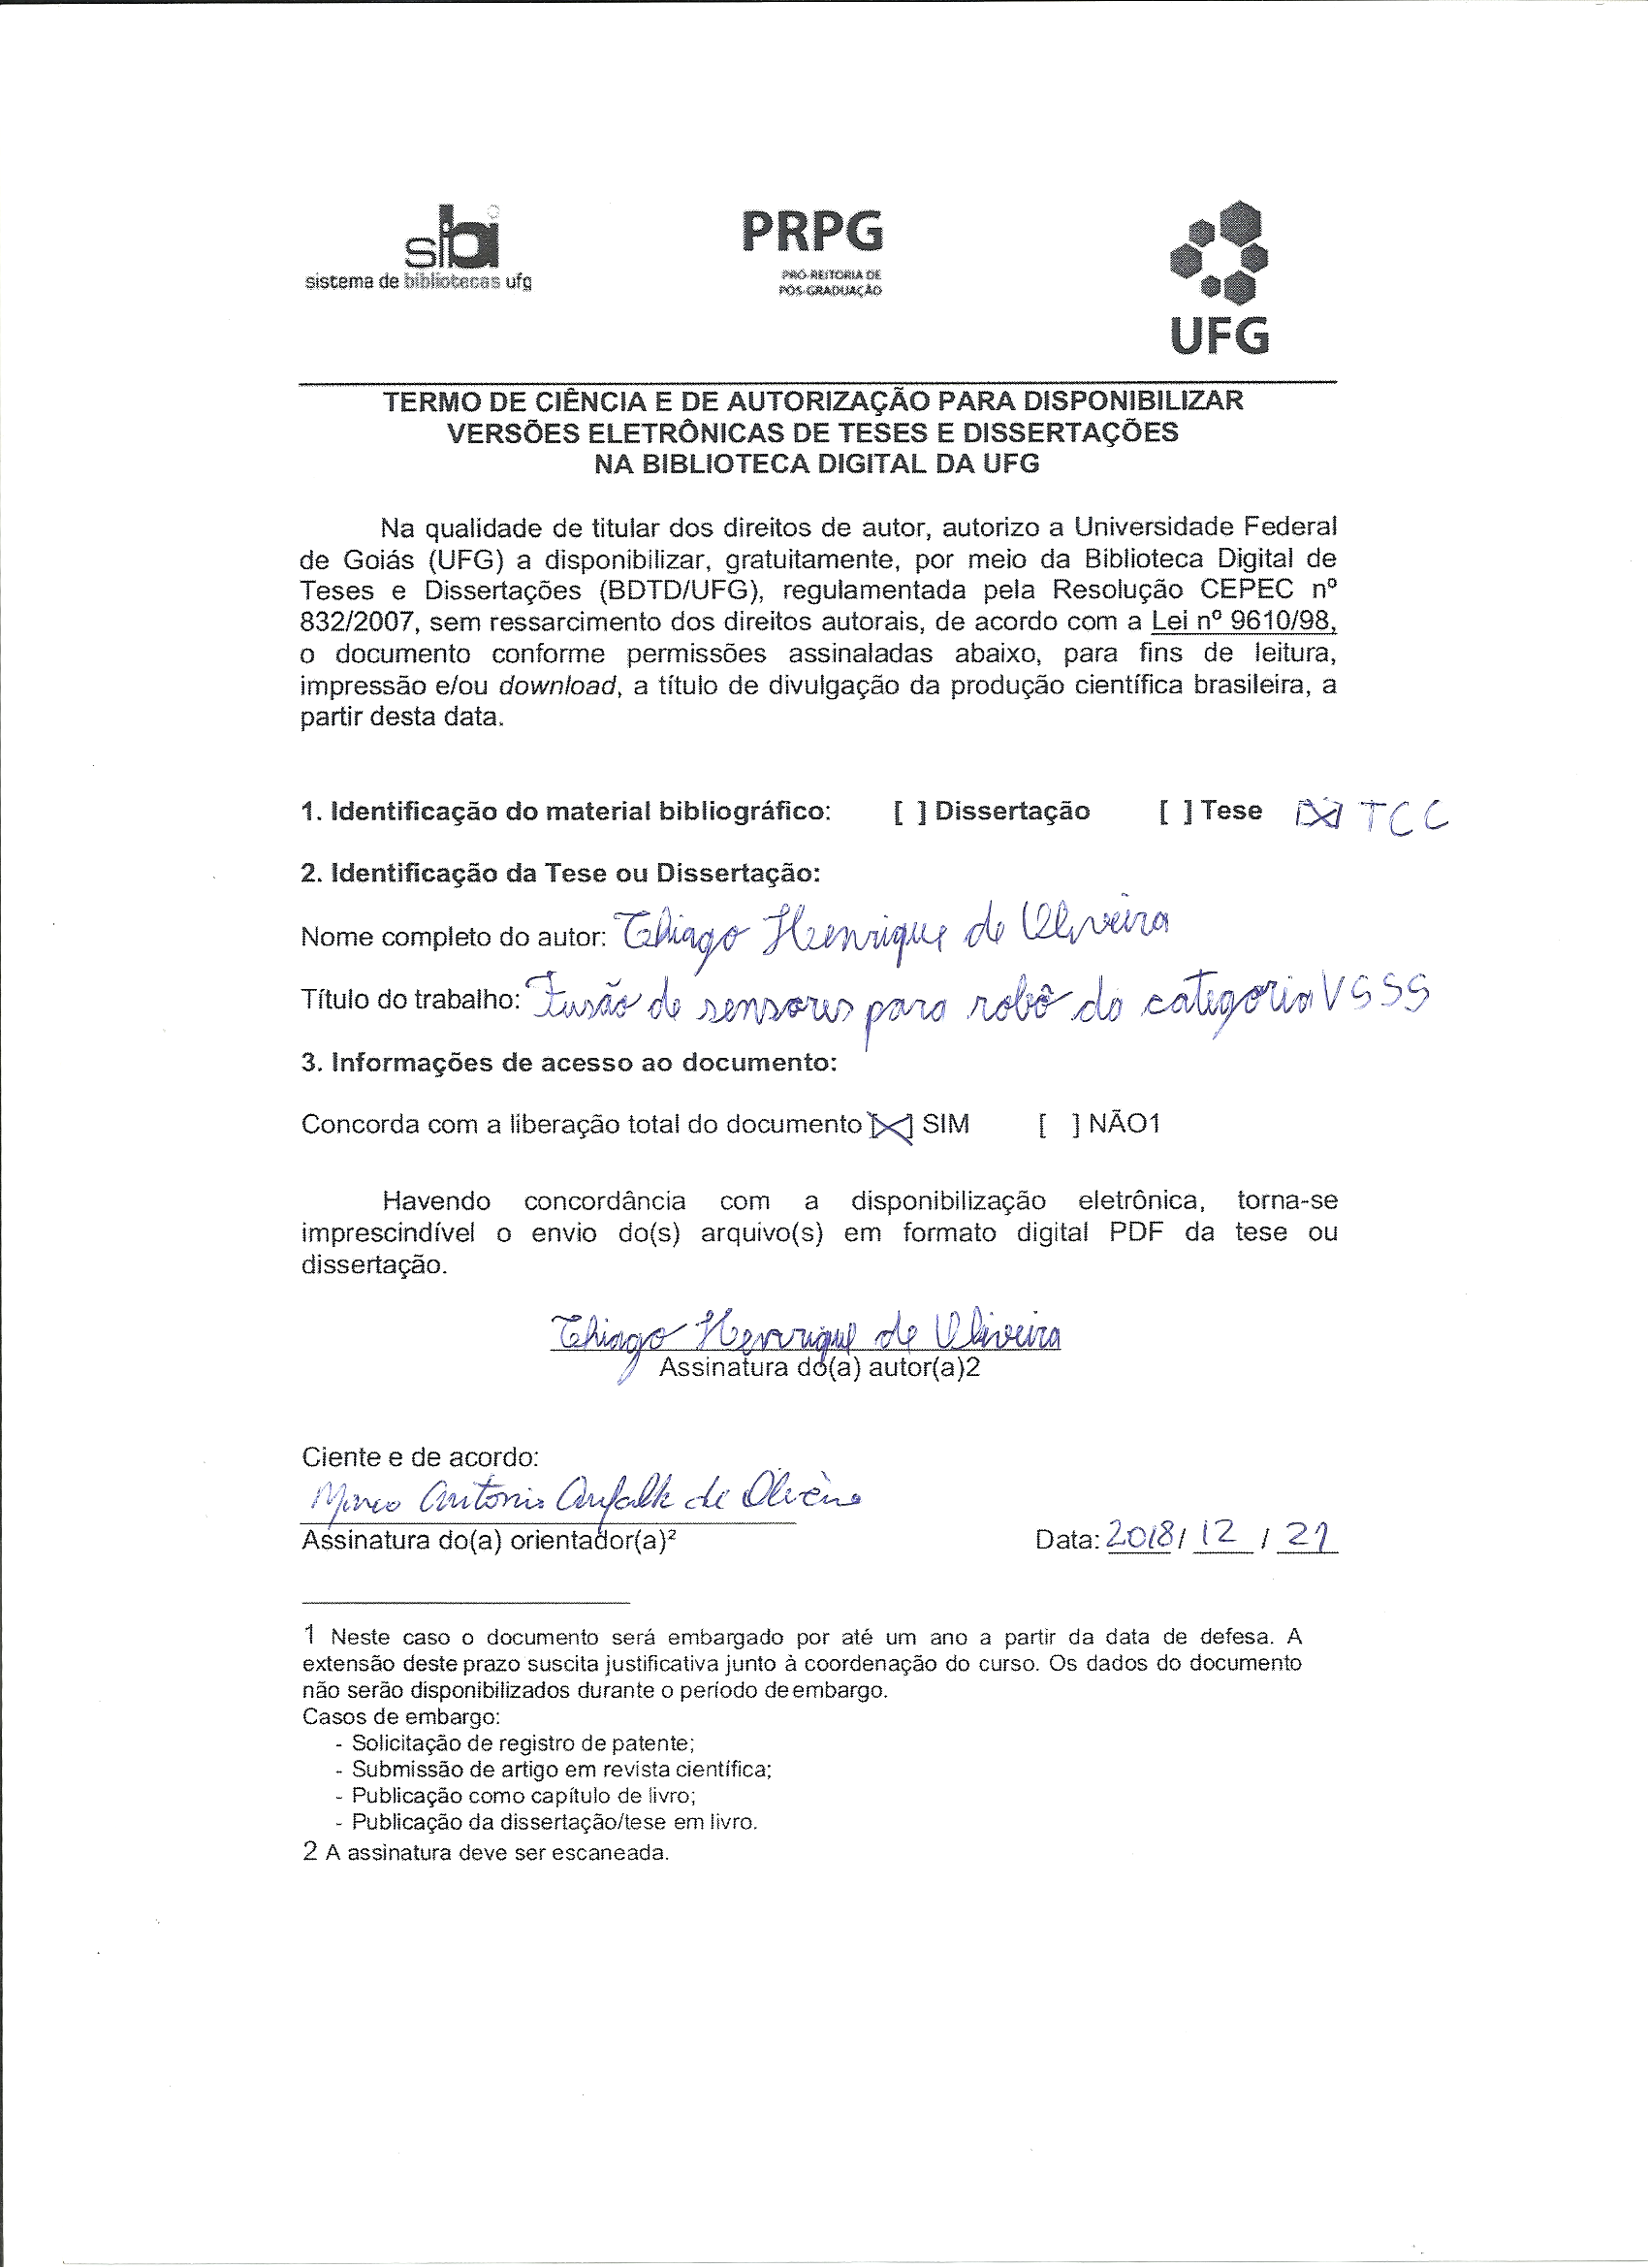
\includepdf{thiago-termo.png}
\imprimirfolhaderosto*
% ---

% ---
% Inserir a ficha bibliografica
% ---

% Isto é um exemplo de Ficha Catalográfica, ou ``Dados internacionais de
% catalogação-na-publicação''. Você pode utilizar este modelo como referência. 
% Porém, provavelmente a biblioteca da sua universidade lhe fornecerá um PDF
% com a ficha catalográfica definitiva após a defesa do trabalho. Quando estiver
% com o documento, salve-o como PDF no diretório do seu projeto e substitua todo
% o conteúdo de implementação deste arquivo pelo comando abaixo:
%
% \begin{fichacatalografica}
%     \includepdf{fig_ficha_catalografica.pdf}
% \end{fichacatalografica}
\begin{fichacatalografica}
	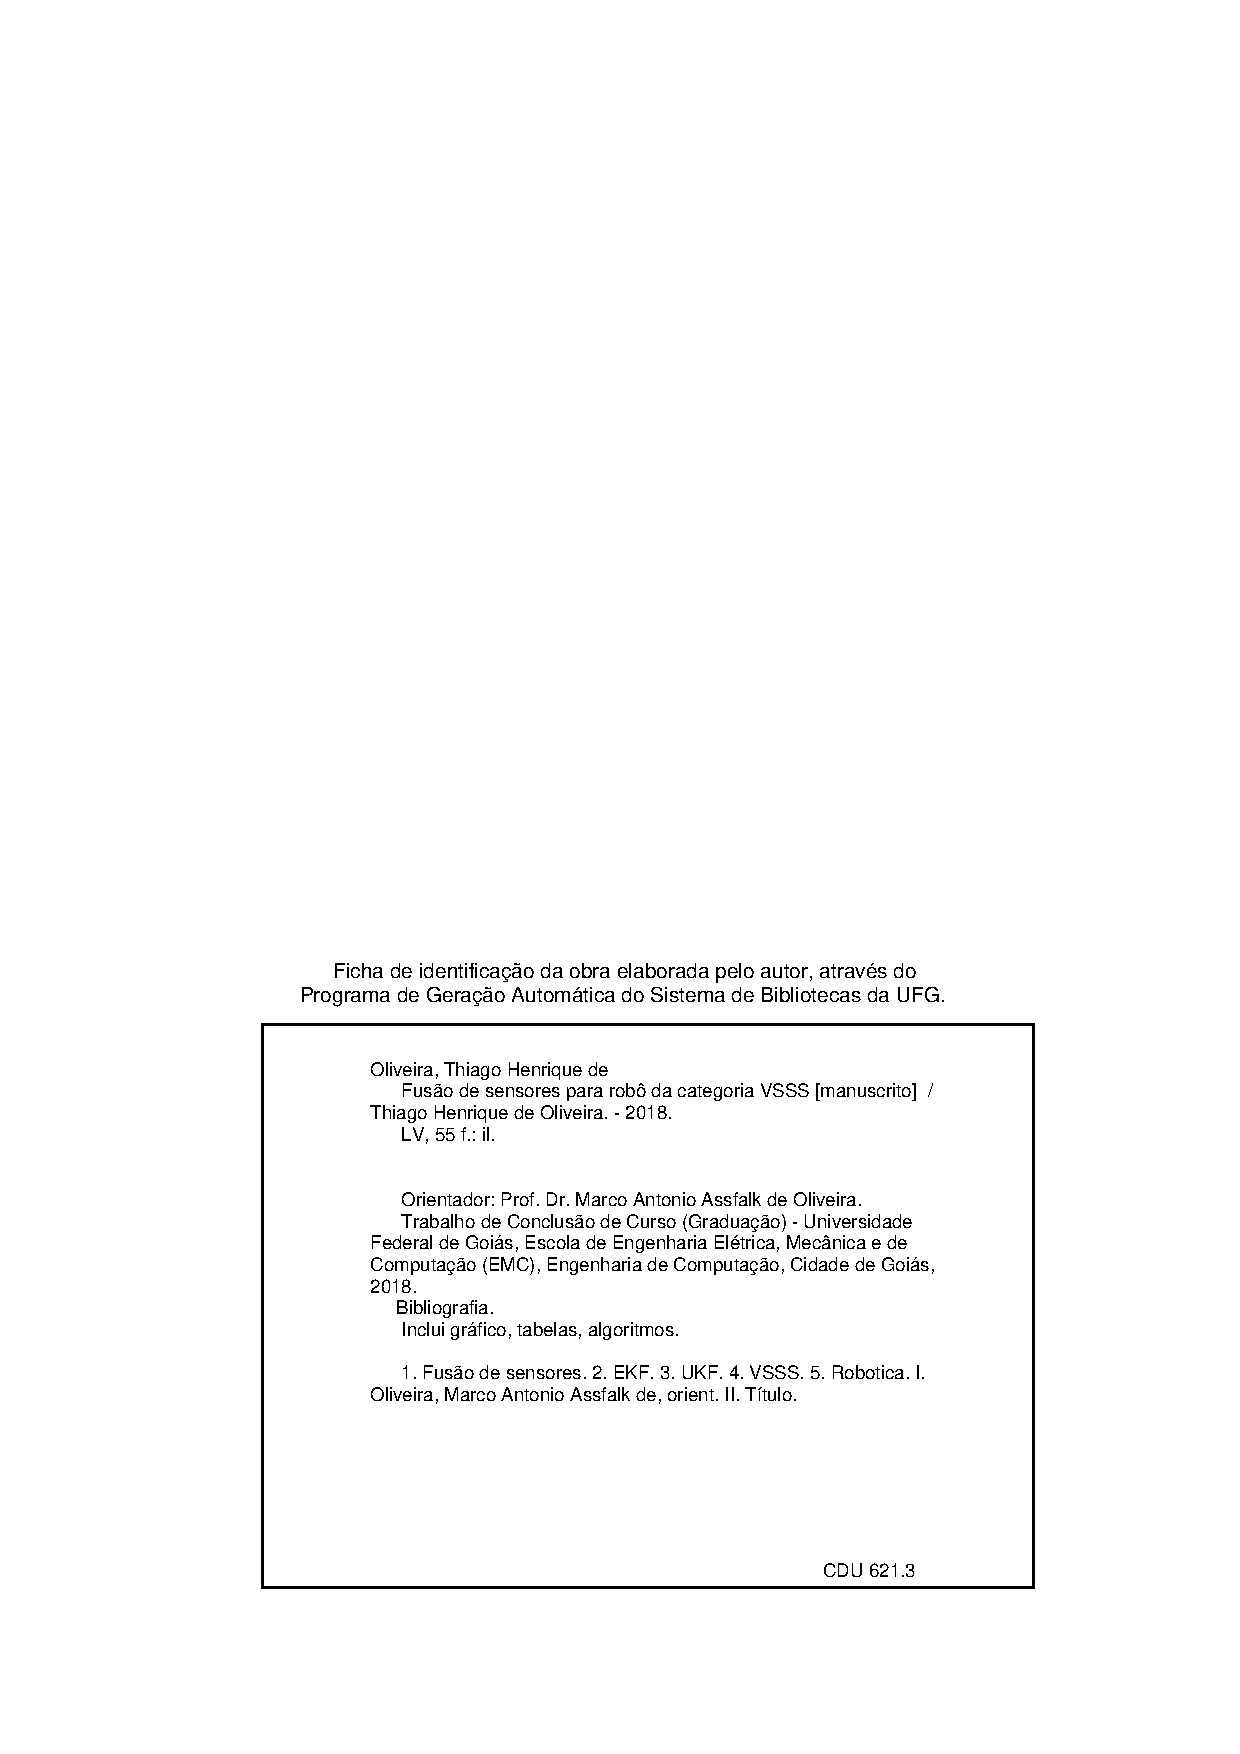
\includepdf{ficha.pdf}
\end{fichacatalografica}

% ---
% Inserir errata
% ---

% ---
% Inserir folha de aprovação
% ---

% Isto é um exemplo de Folha de aprovação, elemento obrigatório da NBR
% 14724/2011 (seção 4.2.1.3). Você pode utilizar este modelo até a aprovação
% do trabalho. Após isso, substitua todo o conteúdo deste arquivo por uma
% imagem da página assinada pela banca com o comando abaixo:
%
% \includepdf{folhadeaprovacao_final.pdf}
%
\begin{folhadeaprovacao}
  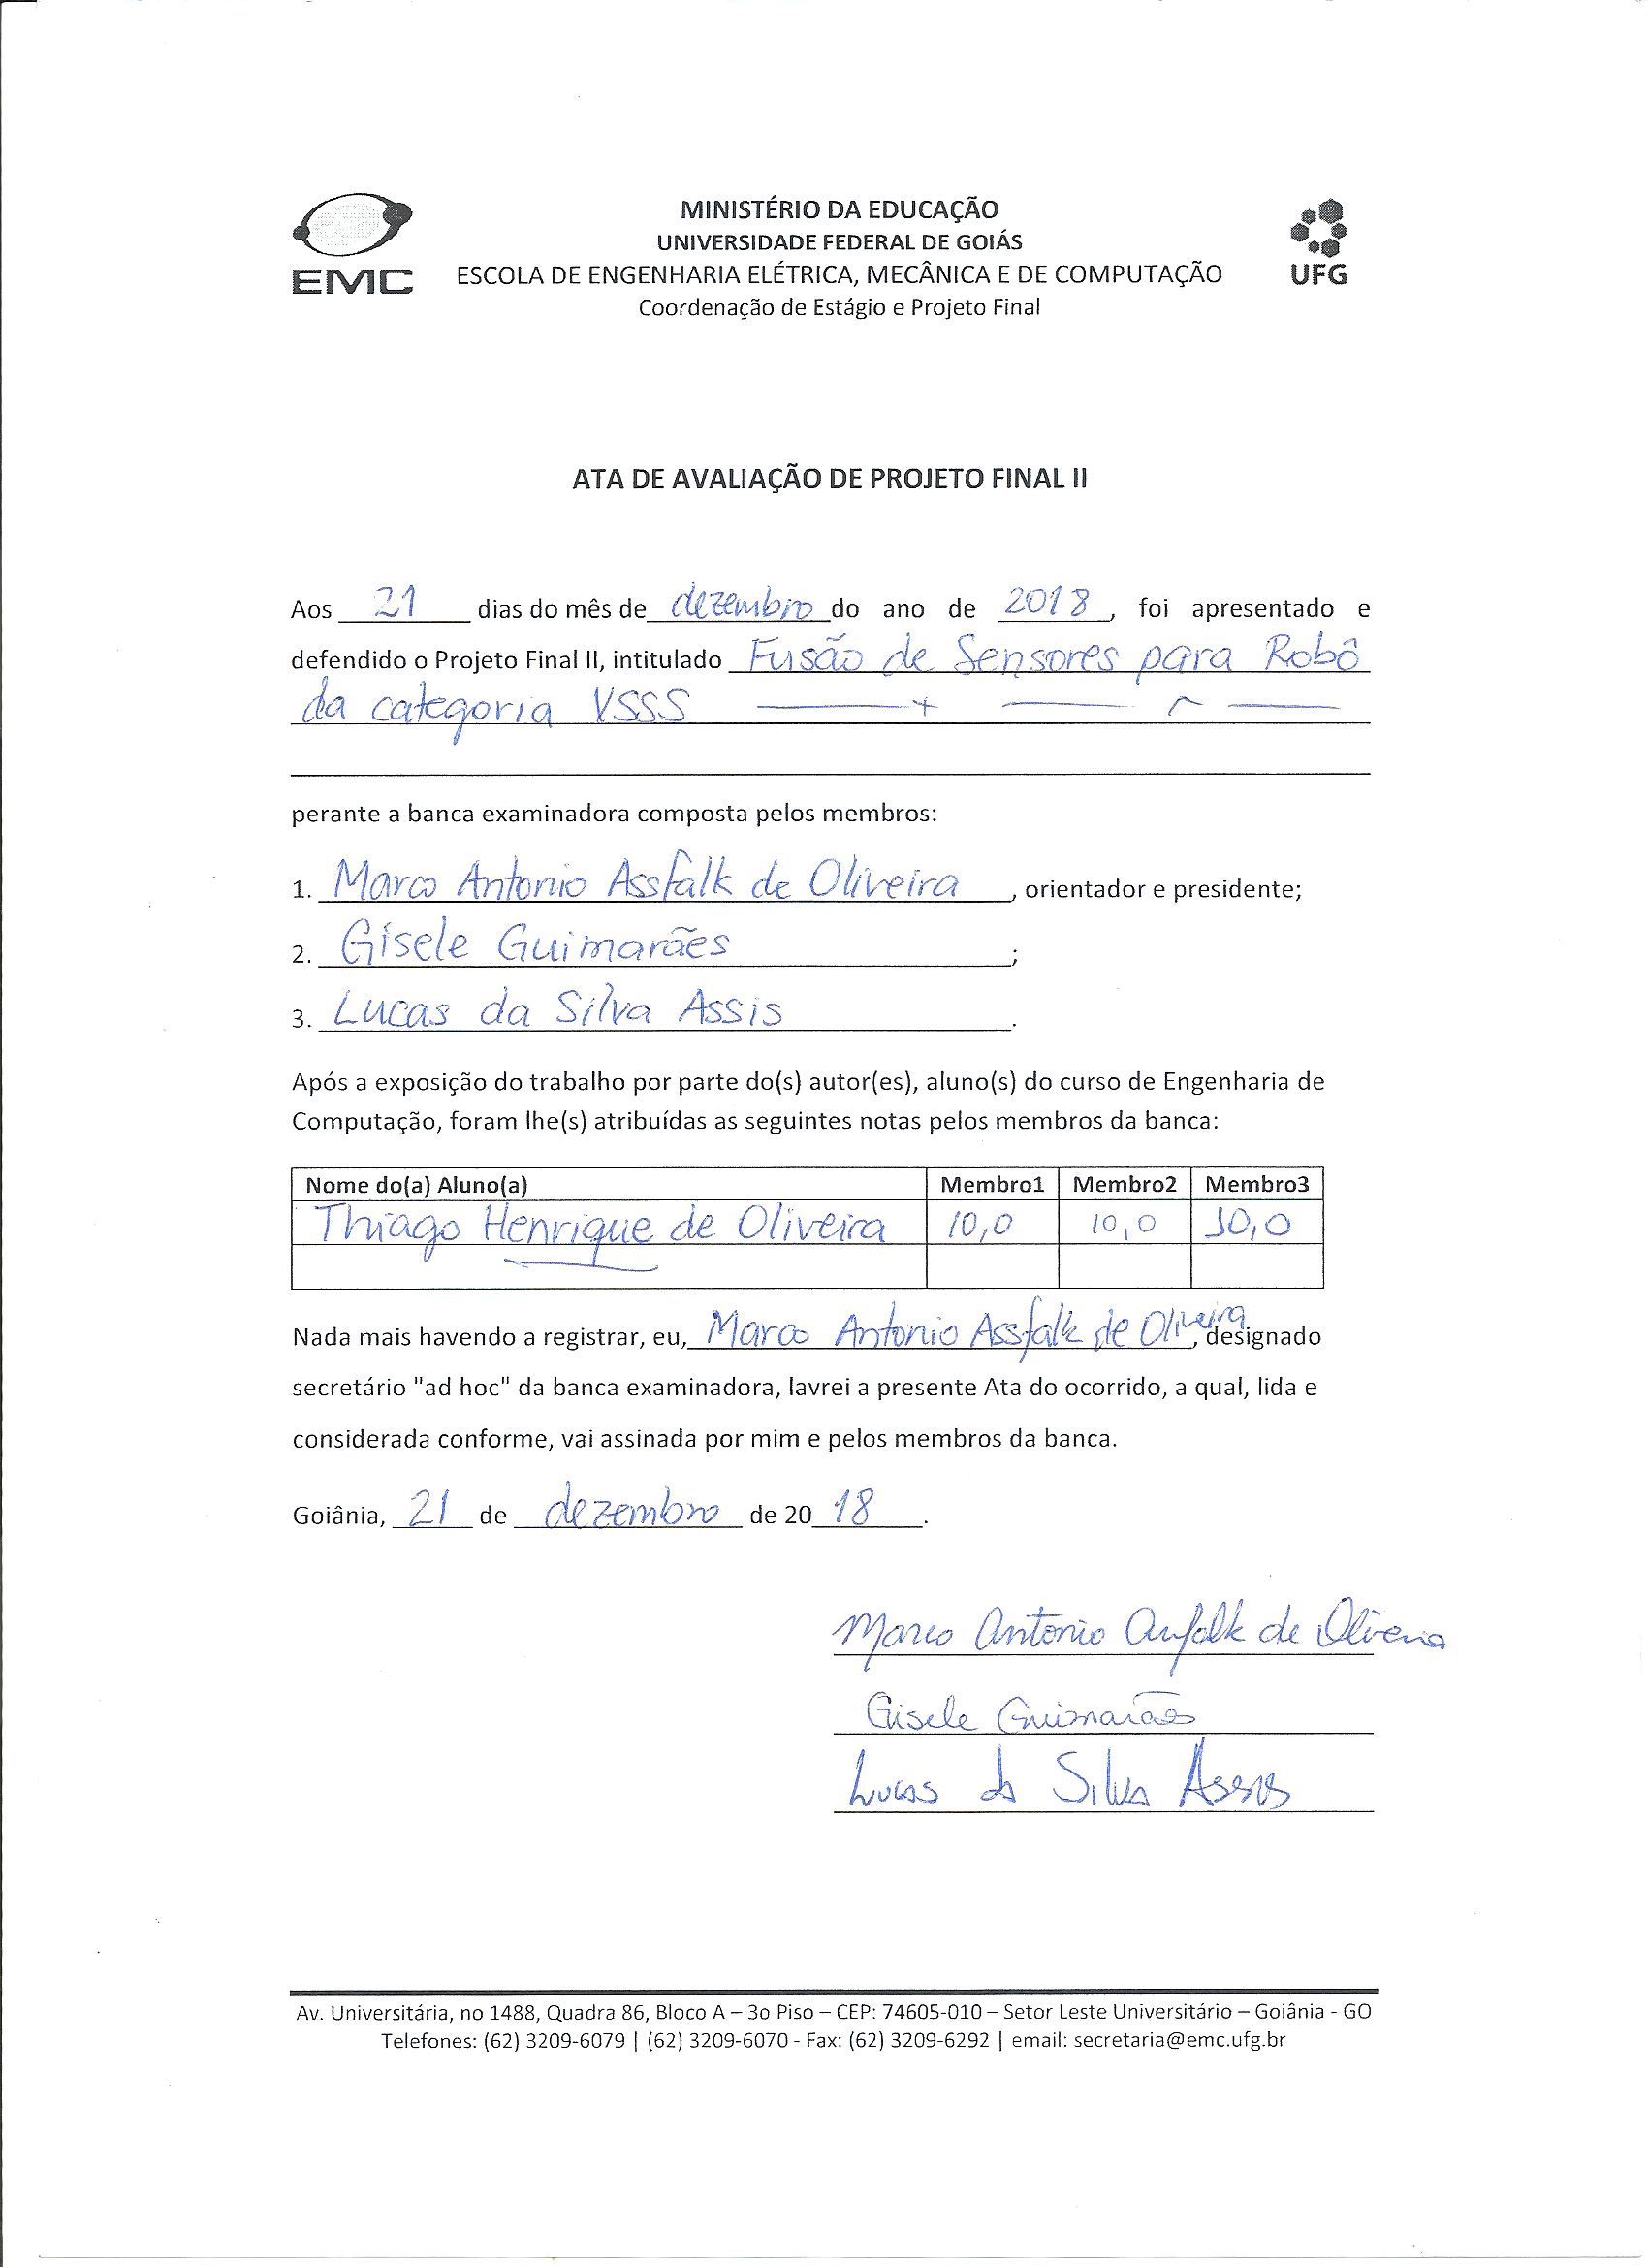
\includepdf{thiago-ata.png}
\end{folhadeaprovacao}

% ---
% RESUMOS
% ---

% resumo em português
\setlength{\absparsep}{18pt} % ajusta o espaçamento dos parágrafos do resumo
\begin{resumo}
\par
IEEE VSSS é uma categoria de competição de robótica em que cada equipe utiliza 3 robôs pequenos, tipicamente de duas rodas, observados por um sistema de visão computacional. Na categoria, os robôs tem o objetivo de jogar futebol, o que exige movimentos rápidos e precisos. Para controlá-los bem, é necessária uma boa estimativa da posição, orientação e velocidade linear e angular. O objetivo deste projeto é estimar bem estas variáveis, utilizando de fusão de sensores para lidar com ruído e falhas inerentes a cada sensor.
\newline
Para obter estes dados, os sensores utilizados foram uma IMU com giroscópio, magnetômetro e acelerômetro de 3 eixos, um encoder em cada roda e um sistema de visão computacional que mede posição e orientação do robô. O Filtro de Kalman Estendido (EKF) foi implementado para combinar a informação desses sensores, modelando a incerteza nas medidas de cada um.
\newline
O Unscented Kalman Filter (UKF) também foi implementado, comparando com o EKF os erros nas estimativas, desempenho de execução e outros fatores importantes.
\newline
Cada sensor foi configurado para medir as variáveis desejadas. Foi encontrado diversas distorções nos sensores, que foram corrigidas utilizando outros sensores como referência e através de métodos estatísticos. Os ruídos de cada um foram medidos e modelados nas matrizes do EKF para atingir uma boa rejeição de ruído.
\newline
Foram feitos vários testes para verificar a qualidade destas estimativas, e o resultado foi satisfatório. Houve boa eliminação de ruído e convergência rápida para o valor correto.

 \textbf{Palavras-chave}: EKF. VSSS. Fusão de sensores.
\end{resumo}


\pdfbookmark[0]{\listfigurename}{lof}
\listoffigures*
\cleardoublepage


% ---
% inserir o sumario
% ---
\pdfbookmark[0]{\contentsname}{toc}
\tableofcontents*
\cleardoublepage
% ---



% ----------------------------------------------------------
% ELEMENTOS TEXTUAIS
% ----------------------------------------------------------
\textual


\chapter{Introdução}
IEEE VSSS é uma categoria de competição de robótica em que cada equipe utiliza 3 robôs pequenos, tipicamente de duas rodas, observados por um sistema de visão computacional. Na categoria, os robôs tem o objetivo de jogar futebol, guiados por um sistema de visão computacional e sensores opcionais dentro do robô. No robô utilizado neste projeto, os sensores disponíveis são uma IMU (unidade de medição inercial) com giroscópio, magnetômetro e acelerometro, um encoder em cada roda e o sistema de visão computacional que mede posição e orientação do robô.
\par
Cada sensor tem vantagens e desvantagens: O giroscópio é rápido e preciso, mas não é capaz de corrigir eventuais erros na orientação por não ser capaz de medi-la diretamente, apenas velocidade angular. O encoder pode medir a velocidade de cada roda separadamente, o o que permite calcular tanto a velocidade linear quanto a angular, mas pode medir dados errados caso o robô derrape. O sistema de visão computacional disponível é capaz de medir posição e orientação diretamente, mas tem baixa taxa de atualização e não tem alta precisão.
\par
Utilizando estes sensores de forma individual em um sistema de controle pode resultar em problemas de estabilidade. Por exemplo, um sistema de controle que utilize realimentação apenas com dados da odometria, mesmo que seja estável em condições normais, pode se tornar instavel caso haja derrapamentos.
\par
Utilizando métodos de fusão sensorial, é possível combinar a informação desses sensores para obter estimativas muito superiores ao que seria obtido de cada um de forma individual. A possibilidade de utilizar sensores diferentes que medem a mesma variável possibilita estimar esta variável com ruído resultante menor do que o ruído de cada sensor individual. É possível levar em consideração o nível de ruído de cada sensor ao combinar os dados obtidos por eles.
\par
O algorítmo utilizado neste projeto é o Filtro de Kalman Estendido (EKF), que modela a incerteza em cada valor medido como um ruído gaussiano, assim como a incerteza na estimativa obtida por ele. Os ruídos de cada um foram medidos e modelados nas matrizes do EKF para que o algorítmo possua boa rejeição de ruído. Cada sensor utilizado foi configurado e as distorções foram corrigidas utilizando outros sensores como referência ou através de métodos estatísticos. Também foi implementado o Unscented Kalman Filter (UKF), para compara-lo com o EKF, observando os erros nas estimativas, desempenho de execução e outros fatores.
\chapter{Desenvolvimento}
\section{Filtro de Kalman Estendido}
Há diversas variações do filtro de Kalman, adequados para sistemas diferentes. O Filtro de Kalman tradicional é compatível apenas com sistemas lineares, então não pode ser utilizado neste sistema. Já o filtro de Kalman estendido (Extended Kalman Filter - EKF) é compatível com sistemas não lineares, e por isso é utilizado neste projeto.
\par
Diferente do Filtro de Kalman tradicional, o filtro de Kalman estendido utiliza equações não lineares para modelar a transição de estados e as medidas, e utiliza jacobianas dessas equações no lugar das matrizes A e B.
\par
O algoritmo é dividido em duas etapas: predição e atualização. Na predição, é calculado o valor das variáveis de estado a partir do valor anterior, utilizando um modelo do sistema para prever os novos valores. Na atualização, os sensores são utilizados para corrigir o valor predito, melhorando a estimativa.
\par
As equações da etapa de predição são:
\begin{equation}
	\bar{\mu_t} = f(\mu _{t-1}, u)
\end{equation}
\begin{equation}
	\bar{\Sigma_t}  = F_t * \Sigma_{t-1} * F_t^T + Q_t
\end{equation}
\par
As equações da etapa de atualização são:
\begin{equation}
	K_t = \bar{\Sigma_t} * H_t^T * (H_t * \bar{\Sigma_t} * H_t^T + R_t)^{-1}
\end{equation}
\begin{equation}
	\mu _t = \bar{\mu} + K_t (z_t - h(\bar{\mu_t}))
\end{equation}
\begin{equation}
	\Sigma _t = (I - K_t * H_t) * \bar{\Sigma_t}
\end{equation}

\par
Em que ${\mu}$ e $\Sigma_t$ são os parâmetros da distribuição normal (valor esperado e matriz de covariança) que modela a estimativa do EKF, u são as variáveis de controle, $\bar{\mu}$ e $\bar{\Sigma_t}$ são os parametros da gaussiana predita pelo modelo, K é o Ganho de Kalman e $z_t$ são os valores medidos pelos sensores.

Para utilizar o algorítmo, devem ser definidas as equações e matrizes:
\begin{itemize}
	\item Modelo do sistema $f(\mu _{t-1}, u)$ e o jacobiano $F_t$
	\item Modelo de medidas $h(\bar{\mu})$ e o jacobiano $H_t$
	\item Matriz de covariancia $R_t$
	\item Matriz de ruído de processo $Q_t$
\end{itemize}

\section{Implementação}
Como o algoritmo deve ser executado em um microcontrolador com processador ARM Cortex-M3, que não possui uma FPU, é necessário que seja implementado de forma altamente otimizada para atingir uma boa taxa de amostragem. O Filtro de Kalman Estendido (e posteriormente, o UKF) foi implementado utilizando a biblioteca Eigen \cite{eigen}, por oferecer operações de matrizes como multiplicação e inversa com alto desempenho. Ela é tipicamente utilizada em computadores x86, mas foi possível compila-la para ARM sem muitos problemas. O tempo gasto para calcular uma iteração do EKF no microcontrolador é de 0.894ms, enquanto o tempo total, incluindo o EKF e a medida de sensores, é de 1.033ms (frequência de 968Hz). O alto desempenho obtido permite tirar bom proveito da alta taxa de atualização dos sensores utilizados.
\par
Outra biblioteca utilizada foi o MBED \cite{mbed}, que fornece um sistema operacional em tempo real (rtos), driver de I2C que foi utilizado para comunicação com os sensores, driver de UART utilizado para comunicar com o rádio xbee, e o driver QEI, que conta os pulsos medidos pelo encoder. Para comunicar com o computador via xbee, foi utilizado a biblioteca XBeeLib \cite{xbeelib} fornecida pela fabricante, que é compatível com o MBED.
\par
A implementação do EKF, drivers dos sensores, modelagem matemática, etc. está disponível no github do Pequi Mecânico \cite{vsss_robot}.

\section{Modelo matemático}
% ---
O movimento do robô pode ser modelado como circular, mas tal modelo resulta equações mais complexas e não definidas para movimentos em linha reta, e por isso não é muito utilizado na literatura. Por isso, o modelo mais comum na literatura, e que é utilizado nesse trabalho, é o do uniciclo \cite{siegwart2004introduction}, em que o movimento é aproximado a uma reta na mesma direção e sentido da velocidade do robô. As equações utilizadas são:
\begin{equation}
	\Delta x = \Delta S * \cos(\theta + \frac{\Delta\theta}{2})
\end{equation}
\begin{equation}
	\Delta y = \Delta S * \sin(\theta + \frac{\Delta\theta}{2})
\end{equation}
A relação entre os deslocamentos e as velocidades linear e angular, para um curto intervalo de tempo, são:
\begin{equation}
	 \Delta S = v * \Delta t
\end{equation}
\begin{equation}
	 \Delta \theta = \omega * \Delta t
\end{equation}
Substituindo na equação anterior, pode se obter a equação de transição de estados:
\begin{equation}
	x_t = x_{t-1} + v_t * \Delta t * \cos(\theta_{t-1} + \frac{\omega_{t} * \Delta t}{2})
\end{equation}
\begin{equation}
	y_t = y_{t-1} + v_t * \Delta t * \sin(\theta_{t-1} + \frac{\omega_{t} * \Delta t}{2})
\end{equation}
\begin{equation}
	\theta_t = \theta_{t-1} + \omega_{t} * \Delta t
\end{equation}
A relação entre as velocidades do robô e a das rodas:
\begin{equation}
	\omega = \frac{(v_r - v_l)}{L}
\end{equation}
\begin{equation}
	 v = \frac{(v_r + v_l)}{2}
\end{equation}
\par
Onde $v_r$ é a velocidade da roda direita e $v_l$ é a velocidade da roda esquerda.
\par
Para poder estimar também as velocidades linear e angular utilizando dados de vários sensores, elas foram consideradas também como variáveis de estado. A variação das velocidades são modeladas pela equação:
\begin{equation}
	v_t = v_{t-1} + a * \Delta t
\end{equation}
\begin{equation}
	\omega_t = \omega_{t-1} + \alpha * \Delta t
\end{equation}
Onde $a$ é a aceleração linear e $\alpha$ é a aceleração angular. Desta forma, as acelerações são as variáveis de controle. Antes de adicionar o acelerômetro, elas eram calculadas numéricamente a partir das velocidades das rodas:
\begin{equation}
	a_{roda} = \frac{v_{t,roda} - v_{t-1,roda}}{T}
\end{equation}
\begin{equation}
	a = \frac{(a_r + a_l)}{2}
\end{equation}
\begin{equation} \label{eq:num_acc}
	\alpha = \frac{(a_r - a_l)}{L}
\end{equation}
\par
A equação \ref{eq:num_acc} foi posteriormente substituida por leituras do acelerômetro presente na IMU utilizada. Para remover a aceleração da gravidade das leituras do acelerômetro, $\theta_y$ foi adicionado como variável de estado para estimar a inclinação do robô no eixo y. A estimativa de $\theta_y$ é descrita em mais detalhes na seção \ref{sec:acc_fix}.
\par
Para eliminar efeitos externos no magnetômetro, $\theta_{offset}$ foi adicionado como variável de estado para estimar o offset nas leituras devido a campos magnéticos não modelados, como a presença de materiais metálicos próximos ao robô. $\omega_y$ foi adicionada como variável de controle para calcular alterações em $\theta_y$. A correção no magnetômetro é descrita em mais detalhes na seção \ref{sec:mag_offset}
\par
O vetor de variáveis de estado é:
\[
\begin{bmatrix}
	x\\
	y\\
	\theta \\
	v\\
	\omega \\
	\theta_{offset} \\
	\theta_y \\
\end{bmatrix}
\]
A equação de transição de estados $f(\mu _{t-1}, u)$ é:
\begin{equation}
	x_t = x_{t-1} + v_{t-1} * \Delta t * \cos(\theta_{t-1} + \frac{\omega_{t-1} * \Delta t}{2})
\end{equation}
\begin{equation}
	y_t = y_{t-1} + v_{t-1} * \Delta t * \sin(\theta_{t-1} + \frac{\omega_{t-1} * \Delta t}{2})
\end{equation}
\begin{equation}
	\theta_t = \theta_{t-1} + \omega_{t-1} * \Delta t
\end{equation}
\begin{equation}
	v_t = v_{t-1} + a * \Delta t
\end{equation}
\begin{equation}
	\omega_t = \omega_{t-1} + \alpha * \Delta t
\end{equation}
\begin{equation}
	\theta_{offset, t} = \theta_{offset, t-1}
\end{equation}
\begin{equation}
	\theta_{y, t} = \theta_{y, t - 1} * \omega_{y, t-1}
\end{equation}
Derivando cada equação em relação a cada variável de estado resulta no jacobiano F:
\begin{equation}
\begin{smallmatrix}
	1 & 0 
	& -v_{t-1} * \Delta t * \sin(\theta_{t-1} + \frac{\omega_{t-1} * \Delta t}{2})
	& \Delta t * \cos(\theta_{t-1} + \frac{\omega_{t-1} * \Delta t}{2}) 
	& -v_{t-1} * \Delta t * \sin(\theta_{t-1} + \frac{\omega_{t-1} * \Delta t}{2}) * \frac{\Delta t}{2} & 0 & 0\\
	0 & 1 
	& v_{t-1} * \Delta t * \cos(\theta_{t-1} + \frac{\omega_{t-1} * \Delta t}{2}) 
	& \Delta t * \sin(\theta_{t-1} + \frac{\omega_{t-1} * \Delta t}{2}) 
	& v_{t-1} * \Delta t * \cos(\theta_{t-1} + \frac{\omega_{t-1} * \Delta t}{2}) * \frac{\Delta t}{2} & 0 & 0\\
	0 & 0 & 1 & 0 & \Delta t & 0 & 0\\
	0 & 0 & 0 & 1 & 0 & 0 & 0\\
	0 & 0 & 0 & 0 & 1 & 0 & 0\\
	0 & 0 & 0 & 0 & 0 & 1 & 0\\
	0 & 0 & 0 & 0 & 0 & 0 & 1\\
\end{smallmatrix}
\end{equation}
\par
O tempo entre dados medidos pela visão computacional é de 33ms devido ao uso de uma câmera de 30fps, enquanto os outros sensores são mais rápidos: giroscópio e acelerômetro suportam taxas de atualização de até 1.66kHz e o magnetômetro de 80Hz. Para lidar com essas diferenças, além de diminuir o tempo gasto calculando o algorítmo, a etapa de atualização foi dividida em duas: utilizar apenas dados da IMU e encoder ou apenas dados da visão e magnetômetro (para correção de offset). Atualizações com IMU e encoder são modelados por uma equação $h(z_t)$ e jacobiano H, enquanto atualizações de visão utilizam $h_v(z_t)$ e $H_v$. A vantagem computacional é grande: as inversas calculadas são de matrizes 4x4, em vez de sempre inverter uma de 7x7.
\par
O modelo de medidas $h(z_t)$ para o IMU e encoder é:
\begin{equation}
	\theta_{magnetometro} = \theta_t + \theta_{offset}
\end{equation}
\begin{equation}
	\omega_{giroscopio} = \omega_t
\end{equation}
\begin{equation}
	v_l = v_t - \frac{\omega_t * L}{2}
\end{equation}
\begin{equation}
	v_r = v_t + \frac{\omega_t * L}{2}
\end{equation}
\par
E o jacobiano H é:
\[
\begin{bmatrix}
	0 & 0 & 1 & 0 & 0 & 1 & 0\\
	0 & 0 & 0 & 0 & 1  & 0 & 0\\
	0 & 0 & 1 & 0 & -\frac{L}{2} & 0 & 0\\
	0 & 0 & 1 & 0 & \frac{L}{2} & 0 & 0\\
\end{bmatrix}
\]
\par
O modelo de medidas $h_v(z_t)$ para a visão é:
\begin{equation}
	x_{visão} = x_t
\end{equation}
\begin{equation}
	y_{visão} = y_t
\end{equation}
\begin{equation}
	\theta_{visão} = \theta_t
\end{equation}
\begin{equation}
	\theta_{mag \, offset \; t} = \theta_{offset \; t}
\end{equation}
\par
E o jacobiano $H_v$ é:
\[
\begin{bmatrix}
	1 & 0 & 0 & 0 & 0 & 0 & 0\\
	0 & 1 & 0 & 0 & 0 & 0 & 0\\
	0 & 0 & 1 & 0 & 0 & 0 & 0\\
	0 & 0 & 0 & 0 & 0 & 1 & 0\\
\end{bmatrix}
\]
\section{Configuração da IMU}

A IMU utilizada \cite{minimu} contém dois circuitos integrados: o LSM6DS33, que contém um giroscópio e um acelerômetro de 3 eixos, e o LIS3MDL, que contém um magnetômetro. A comunicação com os sensores é feita através do protocolo I2C, permitindo ler ou escrever nos registradores internos dos sensores.
\par
De acordo com o datasheet, para escrever em registradores deve ser enviado o endereço do registrador seguido do valor a ser escrito. O datasheet também descreve a funcionalidade de cada um e como configurá-los.
\par
Os registradores relevantes e suas configurações são:

\begin{itemize}
   \item 
   CTRL1\_C: Permite habilitar ou desabilitar cada eixo do giroscópio. Foi inicialmente configurado para habilitar apenas o eixo z, por ser o único necessário para medir a velocidade angular em um sistema de coordenadas 2D. Para corrigir os efeitos da aceleração da gravidade no acelerômetro, o eixo y foi habilitado posteriormete para uso na estimativa de inclinação do robô
   \item
   CTRL2\_G: Permite selecionar a taxa de atualização do giroscópio e valor máximo. A taxa de atualização selecionada foi de 833Hz, que resulta num período de 1.2ms. Períodos menores não são necessários porque as medidas não seriam utilizadas, já que cada etapa do EKF demora aproximadamente 1ms para serem calculadas. Já o valor máximo selecionado foi de $2000\degree$ por segundo, ou 34.9 rad/s, que é o máximo permitido pelo sensor. Valores menores resultariam em saturações, porque o robô conseguiria se movimentar a velocidades angulares maiores que o sensor mede.
   	\item
   	CTRL\_REG2: Configura a faixa de valores que o magnetômetro irá medir. Foi configurado para -4 a +4 Gauss, que é a menor faixa possível, porque a intensidade de campo magnético da terra é menor que 4 Gauss, e faixas menores permitem precisão maior nas medidas.
	\item
	CTRL\_REG1: Configura a taxa de atualização do magnetômetro e habilita os eixos do sensor. Como o robô se movimenta em duas dimensões, foram habilitados apenas os eixos x e y necessários para calcular o ângulo do robô no eixo z. A taxa de atualização foi selecionada como 80Hz (período de 12.5ms) por ser a maior frequência possível. Como o período do sensor é maior que o tempo de calcular o EKF, algumas iterações do EKF não utilizarão o magnetômetro.
	\item
	CTRL9\_XL: Habilita cada eixo do acelerômetro. Foi configurado para habilitar os 3 eixos.
	\item
	CTRL1\_XL: Configura a taxa de atualização e a faixa de medida dos acelerômetro.  A taixa de aceleração disponível é até 6.66kHz. Foi selecionado 1.66kHz, por ser a maior taxa disponível que o microcontrolador consegue processar. A faixa do acelerômetro selecionada é de 4 vezes a aceleração da gravidade (39.2266 $m/s^{2}$), por ser suficiente para atender a aceleração do robô durante o seu movimento.
\end{itemize}
\par
Cada eixo de cada sensor possui dois registradores de 8 bits, que armazenam o byte superior e o inferior da última medição do sensor, que é um número de 16 bits. Para lê-los, é enviado por I2C o endereço do registrador referente ao eixo, seguido do número de bytes que serão lidos, e o sensor responde com o valor armazenado nele.
\par
Com o algoritmo de configurar os sensores e ler os dados pronto, falta apenas converter o valor lido para a unidade de medida correta. Para isso, é utilizado o valor máximo possível de cada sensor, conforme configurado anteriormente. A equação de conversão é:
\begin{equation}
	valor_{real} = valor_{medido} * \frac{valorMáximo_{real}}{valorMáximo_{medido}}
\end{equation}
Como todos os valores são de 16 bits, o $valorMáximo_{medido}$ é sempre:
\begin{equation}
	\frac{2^{16}}{2} - 1 = 32767
\end{equation}
Já o valor máximo real depende de cada sensor.
No giroscópio, como a velocidade angular máxima é de 34.9 rad/s, o valor medido em rad/s é dado por:
\begin{equation}
	\alpha = valor_{medido} * \frac{34.9 rad/s}{32767}
\end{equation}
Já no magnetômetro, como o valor máximo da intensidade de campo magnético foi comfigurado para 4 Gauss, o valor em Gauss é dado por:
\begin{equation}
	B = valor_{medido} * \frac{4 Gauss}{32767}
\end{equation}
E no acelerômetro, com o valor máximo de 39.2266 $m/s^{2}$, o valor medido em $m/s^{2}$ é dado por:
\begin{equation}
	a = valor_{medido} * \frac{39.2266 m/s^{2}}{32767}
\end{equation}
\section{Calibração do giroscópio}
Medindo a velocidade angular através do giroscópio com o robô parado resulta no seguinte gráfico:
\begin{figure}[H]
	\caption{Velocidade angular medida pelo giroscópio com robô parado}
	\begin{center}
   		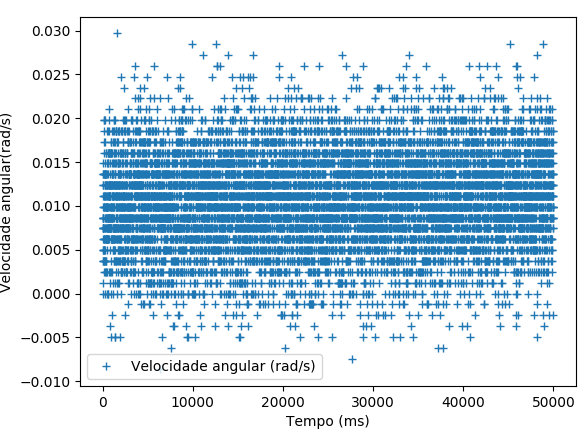
\includegraphics[width=0.7\textwidth]{gyro_parado}
	\end{center}
\end{figure}
O valor médio não é zero, indicando a existência de um offset. Ao medir vários valores do offset e fazer média entre eles, o offset estimado é de 0.01064 rad/s. O offset é corrigido pela equação:
\begin{equation}
	\omega = \omega_{\mathrm{medido}} - \mathrm{offset}
\end{equation}
Entretanto, o offset não é sempre o mesmo, e por isso esta correção deve ser sempre realizada antes de utilizar o robô. Isso pode ser feito realizando amostras e calculando a média delas imediatamente após o robô ser ligado, enquanto ele está parado. Medindo $\omega $ novamente, utilizando a correção proposta:
\begin{figure}[H]
	\caption{Velocidade angular com correção de offset, com o robô parado}
\begin{center}
   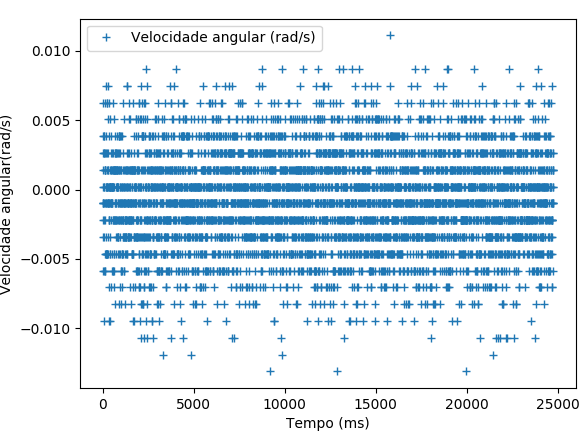
\includegraphics[width=0.7\textwidth]{gyro_parado_auto_fix}
\end{center}
\end{figure}
A média das leituras é aproximadamente 0 rad/s, o que indica que a correção foi bem sucedida. 
\par
Para testar o giroscópio, a velocidade angular medida por ele foi utilizada para calcular orientação, utilizando a equação:
\begin{equation}
	\theta_t = \theta_{t-1} + (\omega_t - \mathrm{offset}) * \Delta t
\end{equation}
Ao girar o robô manualmente em $90\degree$, foi observado o seguinte resultado:
\begin{figure}[H]
	\caption{Orientação calculada ao girar $90\degree$}
\begin{center}
   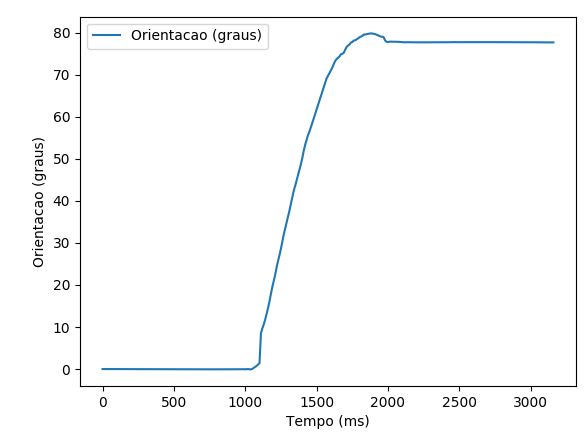
\includegraphics[width=0.7\textwidth]{gyro_90_graus}
\end{center}
\end{figure}
O ângulo calculado no final do movimento foi de apenas 77 graus, o que indica que há alguma distorção na velocidade angular medida pelo giroscópio. Para descobrir que tipo de distorção está presente, os valores de velocidade angular foram medidos através do giroscópio e dos encoders enquanto o robô girando com velocidade crescente, com velocidade das rodas entre 0m/s e 1.15m/s . O resultado obtido foi:
\begin{figure}[H]
	\caption{Velocidade angular medido por giroscópio e encoder}
\begin{center}
   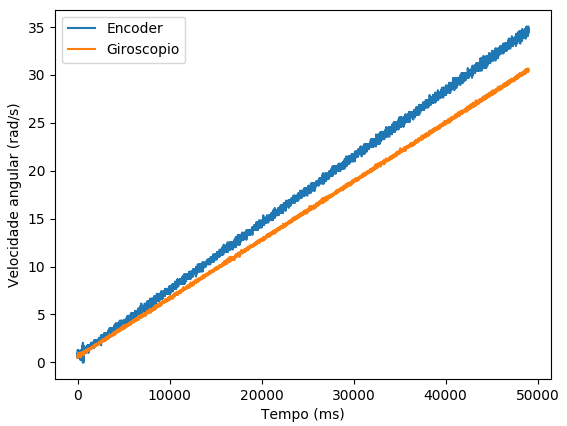
\includegraphics[width=0.7\textwidth]{gyro_enc_comparacao}
\end{center}
\end{figure}
Pode-se perceber que há uma distorção linear no giroscópio, que resulta em medições menores que as reais. A distorção pode ser causada por imperfeições no sensor, eixo z não alinhado perfeitamente com eixo do robô, entre outros.
\par
Para corrigir o problema, foi feito regressão linear nos valores medidos dos dois sensores, o que resultou nos seguintes coeficientes lineares:
\begin{center}
\begin{tabular}{ | l | l | l | p{5cm} |}
    \hline
    Sensor & Coeficiente linear \\ \hline
    Encoder & 0.00346722 \\ \hline
    Giroscópio & 0.00298599 \\
    \hline
\end{tabular}
\end{center}
Estes valores foram então utilizados para corrigir a escala do giroscópio, calculando a velocidade angular correta por:
\begin{equation}
	\omega = \omega_{medido} * \frac{coeficiente_{encorder}}{coeficente_{giroscopio}}
\end{equation}
Repetindo a mesma medição, mas calculando a velocidade angular utilizando a correção definida anteriormente, resulta em:
\begin{figure}[H]
	\caption{Velocidade angular medido por giroscópio e encoder, após a correção}
\begin{center}
   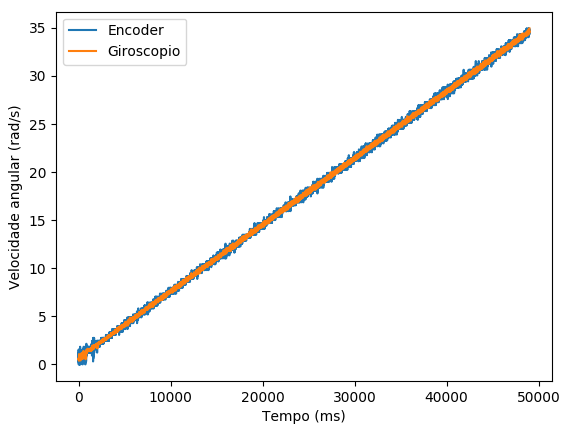
\includegraphics[width=0.7\textwidth]{gyro_enc_comparacao_fix}
\end{center}
\end{figure}
As medidas dos dois sensores se alinharam, demonstrando que a distorção no giroscópio foi corrigida. Ao girar o robô em 90 graus, calculando o ângulo através das medições corrigidas do giroscópio, resultou no gráfico:
\begin{figure}[H]
	\caption{Orientação calculada ao girar $90\degree$, com correção da velocidade angular}
\begin{center}
   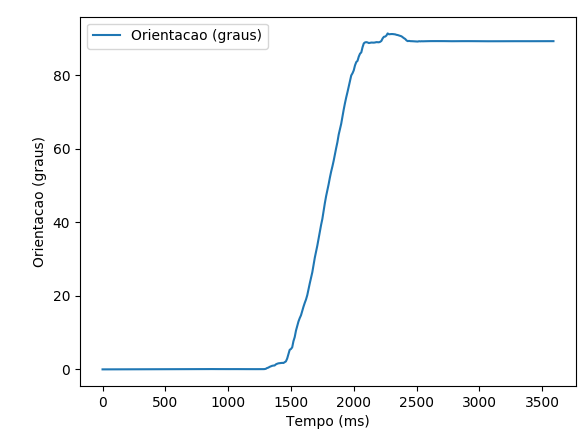
\includegraphics[width=0.7\textwidth]{gyro_90_graus_fix}
\end{center}
\end{figure}
Desta vez o sensor foi capaz de obter o ângulo correto, o que indica que o giroscópio está funcionando corretamente e pode ser incorporado na estimativa de ângulo da fusão de sensores.

\section{Calibração do magnetômetro}
O valor medido pelo magnetômetro é a intensidade do campo magnético da terra, sendo necessário uma forma de calcular a orientação do robô a partir destas medições. Além disso, podem haver distorções no valor medido devido a partes metálicas e magnéticas no robô e devido a imperfeições no sensor, que devem ser corrigidas antes de serem utilizadas.
Para calcular o ângulo, é utilizada a equação:
\begin{equation}
	\theta = \arctan{\frac{-B_y}{B_x}}
\end{equation}
Em que $B_x$ e $B_y$ são as intensidades do campo magnético nos eixos x e y.
\par
Para observar possíveis distorções nos valores medidos, o robô foi girado continuamente em torno do próprio eixo, enquanto o magnetômetro media a intensidade do campo magnético nos eixos x e y. Ao traçar os valores dois dois eixos, o resultado é o seguinte:
\begin{figure}[H]
	\caption{Elipse formada pelas medidas nos eixos x e em y do magnetômetro}
\begin{center}
   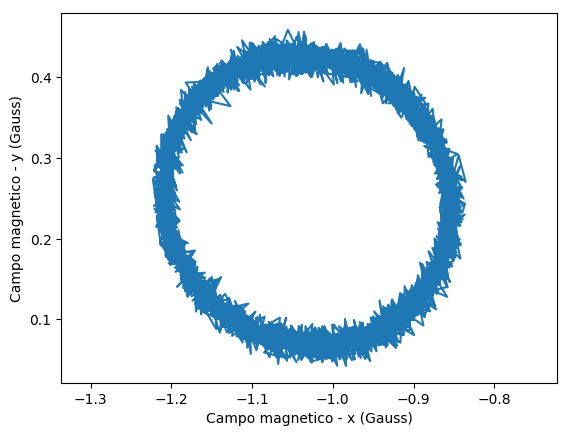
\includegraphics[width=0.7\textwidth]{mag_x_y}
\end{center}
\end{figure}
Através do gráfico pode-se perceber que o centro do círculo não está na origem, o que indica a presença de um offset. Também é visível que o eixo y está um pouco mais alongado que o eixo x, exigindo a normalização dos valores.
O valor real do campo magnético foi modelado como:
\begin{equation}
	B = \frac{B_{medido}}{B_{máximo}} - \mathrm{offset}
\end{equation}
O offset elimina o efeito das partes metálicas e magnéticas no robô, enquanto a divisão pelo valor máximo normaliza as medidas, corrigindo diferenças de escala entre os eixos x e y do sensor. Desta forma, os valores medidos estão sempre entre 0 e 1. Zero significa que o eixo está perpendicular ao campo magnético da terra, e 1 significa que está alinhado com o campo.
\par
O valor máximo e média de cada eixo no teste anterior é:
\begin{center}
\begin{tabular}{ | l | l | l | p{5cm} |}
    \hline
    Eixo & Valor máximo & média \\ \hline
    x & 0.1877037 & -1.02949175 \\ \hline
    y & 0.1946520 & 0.24693936 \\
    \hline
\end{tabular}
\end{center}
O offset de cada eixo é a média dos valores medidos. Ao realizar o mesmo experimento, aplicando a correção descrita acima, foi obtido o seguinte gráfico:
\begin{figure}[H]
	\caption{Elipse formada pelas medidas nos eixos x e em y do magnetômetro, após correções}
\begin{center}
   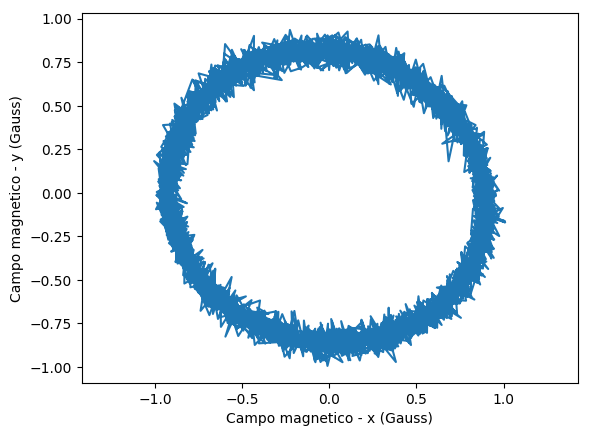
\includegraphics[width=0.7\textwidth]{mag_x_y_fix}
\end{center}
\end{figure}
O raio do círculo é 1 e o centro está na origem, indicando que a correção foi bem sucedida.
\par
Ao mover o robô aproximadamente a $90\degree$ e voltá-lo a orientação original, a orientação medida foi:
\begin{figure}[H]
	\caption{Orientação do robô medida pelo magnetômetro}
\begin{center}
   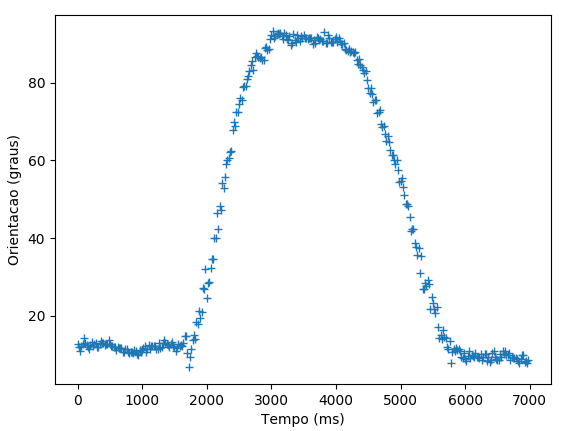
\includegraphics[width=0.7\textwidth]{mag_90_teste}
\end{center}
\end{figure}
O angulo foi medido corretamente, confirmando que o modelo utilizado é capaz de corrigir os problemas detectados.

\section{Offsets do magnetômetro}\label{sec:mag_offset}
Uma das desvantagens dos magnetômetros é que, como eles medem a intensidade do campo magnético, qualquer objeto metálico ou magnético interfere em suas leituras. Isso se torna um problema quando o robô deve ser utilizado próximo de outros robôs, como é o caso da aplicação estudada neste trabalho. Por isso, é necessário uma forma de impedir que estas interferências resultem em um erro na estimativa da orientação do robô.
Para observar interferências, foi medido a orientação calculada por dados do magnetômero do robô parado, enquanto outro robô foi aproximado e afastado dele.
\begin{figure}[H]
	\caption{Orientação do robô medida pelo magnetômetro devido a interferências}
\begin{center}
   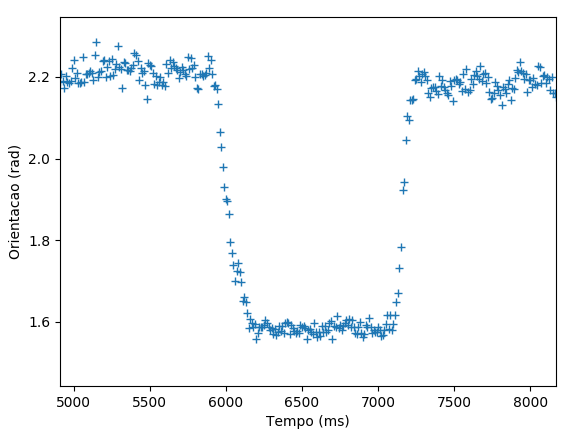
\includegraphics[width=0.7\textwidth]{theta_offset}
\end{center}
\end{figure}
Para resolver este problema, o offset do magnetômetro foi adicionado as variáveis de estado do robô, para que o EKF possa estimá-lo.
Dessa forma, o modelo de medida para leituras do magnetômetro passa a ser:
\begin{equation}
	\theta_{mag} = \theta + \theta_{offset}
\end{equation}
E ao ter dados da visão computacional disponíveis, o magnetômetro é lido e $\theta_{offset}$, calculado pela equação e utilizado na etapa de atualização do EKF:
\begin{equation}
	\theta_{offset} = \theta_{mag} - \theta_{visao}
\end{equation}
Dessa forma, a visão computacional contribui com a estimativa do offset do magnetômetro.
Com a correção de interferências externas implementada, foi estimar a orientação do robô. No gráfico a seguir, o robô foi movimentando manualmente, e em seguida, outro robô foi aproximado dele. Foi obtido os resultados:
\begin{figure}[H]
	\caption{Orientação do robô medida pelo magnetômetro, com e sem correção}
\begin{center}
   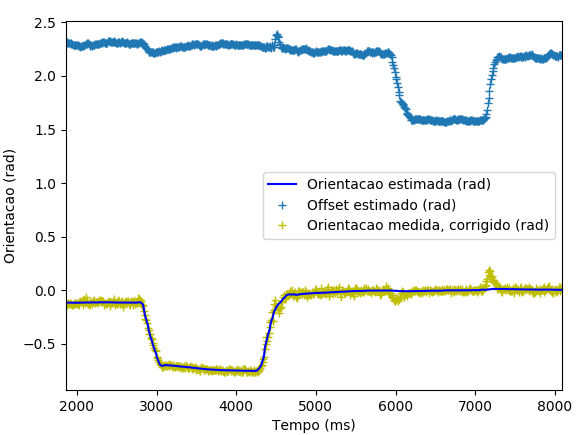
\includegraphics[width=0.8\textwidth]{mag_offset_fix}
\end{center}
\end{figure}
Nesse gráfico, pode-se observar que apesar de as leitudas do magnetômetro terem sido afetadas pelo outro robô, a orientação estimada continuou correta, ignorando as influências externas.

\section{Correções no acelerômetro}\label{sec:acc_fix}
Deixando o robô parado, o acelerômetro mede a aceleração da gravidade:
\begin{center}
\begin{tabular}{ | l | l | l | p{5cm} |}
    \hline
    eixo & aceleração $(m/s^2)$ \\ \hline
    $a_x$ & -0.525424 \\
    $a_y$ & 0.402307 \\
    $a_z$ & 9.774617 \\
    $ \sqrt{a_x^2+a_y^2+a_z^2} $ & 9.796992 \\
    \hline
\end{tabular}
\end{center}
O robô pode se inclinar no eixo y, o que influencia nas medidas de aceleração dos eixos x e z. Inclinando o robô ao máximo, a aceleração medida foi:
\begin{center}
\begin{tabular}{ | l | l | l | p{5cm} |}
    \hline
    eixo & aceleração $(m/s^2)$ \\
    $a_x$ & 0.105287 \\
    $a_y$ & 0.406665 \\
    $a_z$ & 9.792763 \\
    $ \sqrt{a_x^2+a_y^2+a_z^2} $ & 9.801768 \\
    \hline
\end{tabular}
\end{center}
Pode-se observar que o modulo da aceleração é quase o mesmo, mas a componente x foi muito alterada devido a mudança no angulo entre o vetor da aceleração da gravidade e o eixo medido pelo sensor. Isso significa que o eixo x não pode ser utilizado diretamente como aceleração do robô, e que também que esse erro não é constante durante o movimento do robô. É necessário levar em consideração a inclinação do robô para corrigi-lo.

Os vetores relevantes podem ser modelados como:
\begin{center}
\begin{tikzpicture}
  \draw[->] (-3,0)--(3,0) node[right]{$x$};
  \draw[->] (0,-3)--(0,3) node[above]{$z$};
  
  \coordinate (o) at (0, 0);
  \coordinate (ag) at (0, 2);
  \coordinate (ar) at (2, 0);
  \coordinate (ax) at (1.12325634, -0.408832);
  \coordinate (az) at (0.8767433, 2.408831);

  \pgfmathanglebetweenpoints
    {\pgfpointanchor{ax}{center}}
    {\pgfpointanchor{ar}{center}}
  \edef\angB{\pgfmathresult}

  \draw[line width=1pt,-stealth]
  	(o)--(ag) node[anchor=south west]{$\vec{a_g}$};
  \draw[line width=1pt,-stealth]
  	(o)--(ar) node[anchor=south west]{$\vec{a_r}$};
  \draw[line width=1pt,-stealth]
  	(o)--(ax) node[anchor=north east]{$\vec{a_x}$};
  \draw[line width=1pt,-stealth]
  	(o)--(az) node[anchor=south west]{$\vec{a_z}$};

  \draw[very thin] (1, 0) arc (0:-\angB:0.9)
  	node[anchor=south west]{$\theta_y$};
     
\end{tikzpicture}
\end{center}
Em que $a_g$ é a aceleração da gravidade, $a_r$ é a aceleração do robô, e $a_x$ e $a_z$ são as acelerações medidas pelos eixos x e z do robô.
Calculando as projeções de $a_g$ e $a_r$ nos eixos $a_x$ e $a_z$ resulta nas equações:
\begin{equation}
	a_x = a_r * \cos{\theta_y} - ag * \sin{\theta_y}
\end{equation}
\begin{equation}
	a_z = a_r * \sin{\theta_y} + ag * \cos{\theta_y}
\end{equation}
E também vale a relação:
\begin{equation}
	\sqrt{a_x^2 + a_z^2} = \sqrt{a_r^2 + a_g^2}
\end{equation}
Mantando o robô parado para que $a_r$ seja 0, é calculado a aceleração da gravidade pela equação:
\begin{equation}
	a_g = \sqrt{a_x^2 + a_z^2}
\end{equation}
E a inclinação do robô é obtida por:
\begin{equation}
	\theta_y = \arccos{\frac{a_z}{a_g}}
\end{equation}
Esses dois valores são calculados sempre que o robô é ligado, para que possam ser utilizados posteriormente para remover o efeito da gravidade em $a_x$, permitindo obter $a_r$. Como a inclinação $\theta_y$ não permanece constante durante todo o movimento do robô, ela é estimada pelo EKF através das medidas do eixo y do giroscópio:
\begin{equation}
	\theta_{y \; t} = \theta_{y \; t-1} + \omega_y * \Delta t
\end{equation}
A partir de $a_x$ medido pelo acelerômetro, $\theta_y$ estimado pelo EKF e $a_g$ medido anteriormente, a aceleração real do robô sem a aceleração da gravidade é calculada:
\begin{equation}
	a_r = \frac{ a_x - a_g * \sin{\theta_y} }{ \cos{\theta_y} }
\end{equation}
Para testar a correção da componente da gravidade, os valores de $a_x$, $a_r$ e $\theta_y$ foram medidos mantendo o robô parado, inclinando o robô manualmente:
\begin{figure}[H]
	\caption{Inclinação do robô e aceleração com e sem correção}
\begin{center}
   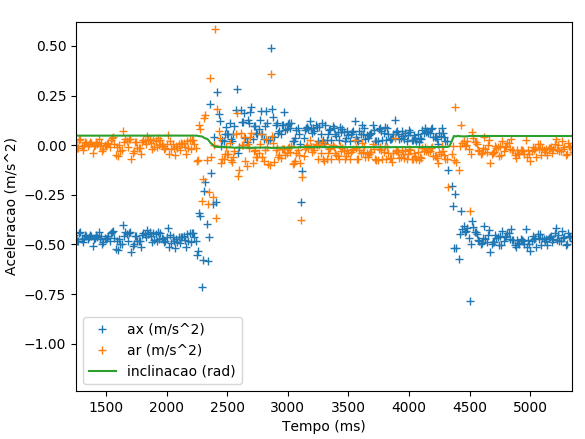
\includegraphics[width=0.7\textwidth]{acc_theta_fix}
\end{center}
\end{figure}
Como é visível no gráfico, enquando houve grandes alterações em $a_x$, a aceleração $a_r$ não é muito influenciada pela inclinação do robô.
\par
Ainda há outras acelerações que modificam o valor lido pelo giroscópio. Ao girar o robô em torno do próprio eixo com velocidade angular de 20 rad/s, o acelerômetro mede uma aceleração adicional nos eixos x e y:
\begin{figure}[H]
	\caption{Aceleração em x e y com rotação constante a 20 rad/s}
\begin{center}
   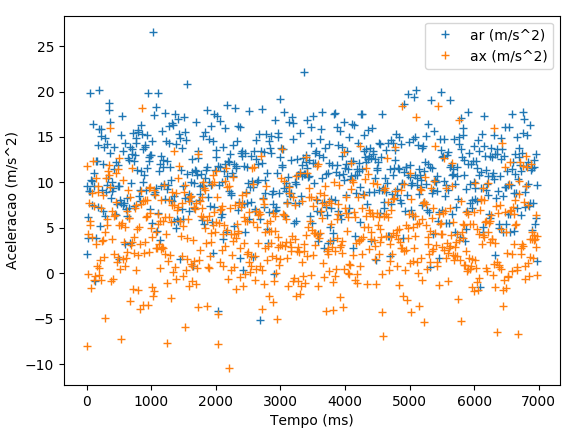
\includegraphics[width=0.7\textwidth]{acc_x_y_spin}
\end{center}
\end{figure}
Os valores medidos de $a_x$ e $a_y$ tem média de 10.8527 e 4.45632 $m/s^2$, respectivamente. Estes valores são componentes da aceleração centrípeta que surgiu devido ao giro do robô. Para saber a aceleração linear na direção do movimento do robô, é preciso removê-la. As acelerações nos eixos x e y foram modeladas como:
\begin{center}
\begin{tikzpicture}
  \draw[->] (-2.5,0)--(2.5,0) node[right]{$a_x$};
  \draw[->] (0,-2.5)--(0,2.5) node[above]{$a_y$};
  
  \coordinate (o) at (0, 0);
  \coordinate (ac) at (2, 1.6);
  \coordinate (at) at (1.5, 1.2);
  \coordinate (acp) at (2, 0);
  \coordinate (ar) at (1.7, 0);

  \pgfmathanglebetweenpoints
    {\pgfpointanchor{o}{center}}
    {\pgfpointanchor{ac}{center}}
  \edef\angA{\pgfmathresult}
  \pgfmathanglebetweenpoints
    {\pgfpointanchor{acp}{center}}
    {\pgfpointanchor{ac}{center}}
  \edef\angB{\pgfmathresult}

  \draw[line width=1pt,-stealth]
  	(o)--(ac) node[anchor=south east]{$\vec{a_c}$};
  	
  	\draw[dashed]
  	(ac)--(acp) node[anchor=south east]{};
  	
  \draw[line width=1pt,-stealth]
  	(o)--(ar) node[anchor=north east]{$\vec{a_r}$};

	\draw[very thin] (at) arc (\angA:\angB:-0.7)
  		node[anchor=south east]{$\theta$};
     
\end{tikzpicture}
\end{center}
em que $a_c$ é a aceleração centrípeta e $a_r$ é a aceleração real do robô. As acelerações no eixo x e y podem ser obtidas pelas equações:
\begin{equation}
	a_x = a_c * \sin{\theta} + a_r
\end{equation}
\begin{equation}
	a_y = - a_c * \cos{\theta}
\end{equation}
A aceleração centrípeta pode ser escrita em função da velocidade angular:
\begin{equation}
	a_c = \omega^2 * r
\end{equation}
E $\omega$ é medido pelo giroscópio. Dessa forma, a aceleração do robô é obtida por:
\begin{equation}
	a_r = a_x - \omega^2 * r * \sin{\theta}
\end{equation}
Girando o robô novamente a velocidade angular de 20 rad/s, medindo a aceleração no eixo x, com e sem correção da aceleração centrípeta:
\begin{figure}[H]
	\caption{ax e ar com rotação constante a 20 rad/s}
\begin{center}
   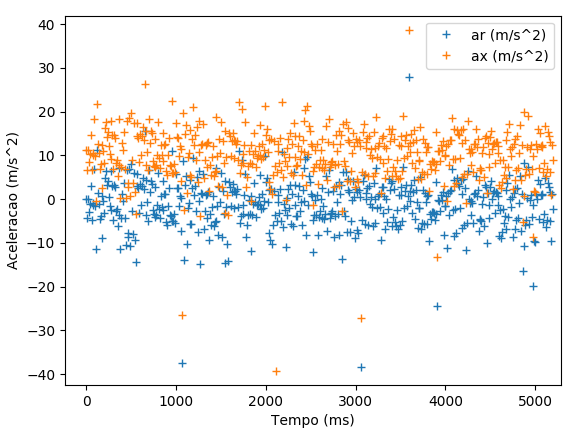
\includegraphics[width=0.7\textwidth]{acc_ax_ar_fix}
\end{center}
\end{figure}
Mostrando que o efeito da aceleração centrípeta na medida da aceleração do robô foi reduzido.

\section{Medida de covariância do encoder e giroscópio}

Para medir a covariância do encoder e giroscópio, aplicou-se 0.5m/s (velocidade típica) na roda direita e -0.5m/s na roda esquerda, o fazendo girar. O robô mediu a velocidade das rodas através do encoder e a velocidade angular através do giroscópio. O resultado foi:
\begin{figure}[H]
	\caption{Velocidade angular e velocidades de cada roda}
\begin{center}
   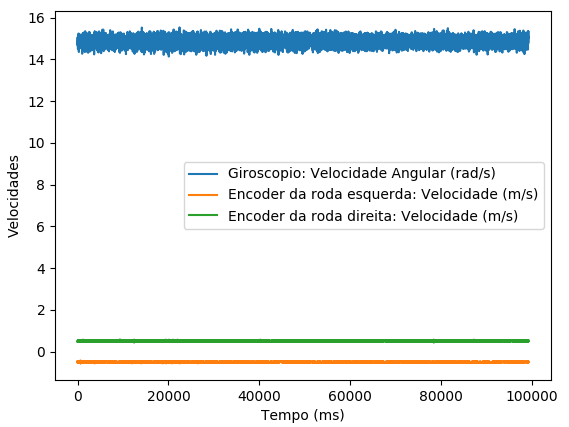
\includegraphics[width=0.7\textwidth]{cov_gyro_enc}
\end{center}
\end{figure}
Utilizando as ferramentas do matplotlib \cite{matplotlib} para montar um histograma e o scipy \cite{scipy} para fazer o fitting em gaussiana dos valores medidos, pode-se observar o ruído do giroscópio:
\begin{figure}[H]
	\caption{Gaussiana do giroscópio}
\begin{center}
   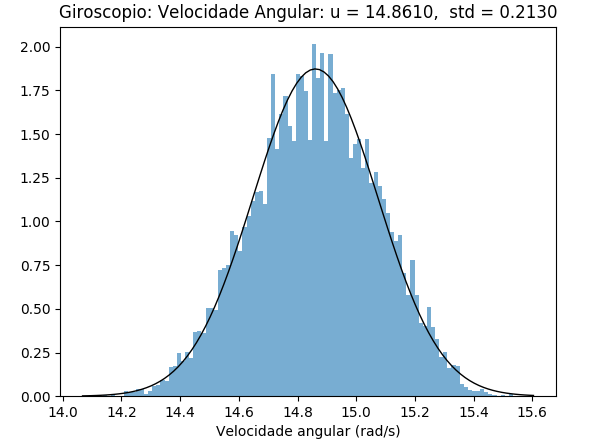
\includegraphics[width=0.7\textwidth]{gyro_gaussiana}
\end{center}
\end{figure}
O que indica que o ruído está muito próximo de um ruído gaussiano. Os histogramas das medidas de velocidade do encoder da roda direita e da esquerda são:
\begin{figure}[H]
  \centering
  \begin{minipage}[b]{0.45\textwidth}
    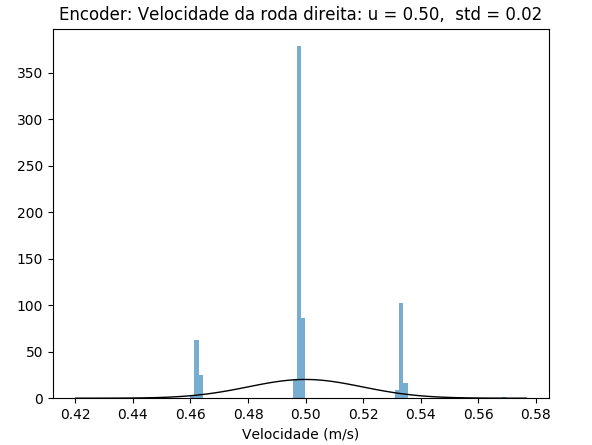
\includegraphics[width=\textwidth]{encoder_roda_direita_gaussiana}
    \caption{Gaussiana do encoder da roda direita}
  \end{minipage}
  \begin{minipage}[b]{0.45\textwidth}
    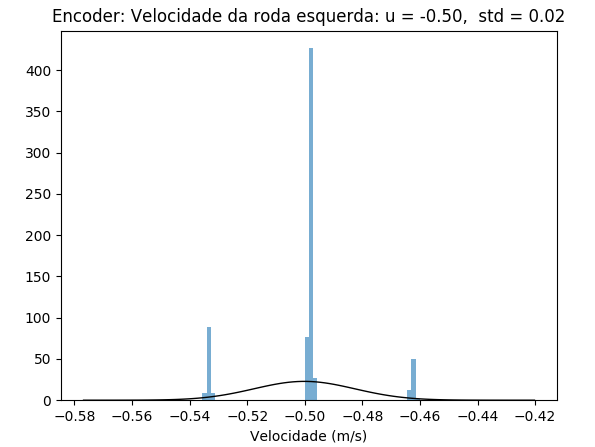
\includegraphics[width=\textwidth]{encoder_roda_esquerda_gaussiana}
    \caption{Gaussiana do encoder da roda esquerda}
  \end{minipage}
\end{figure}
Neste gráfico pode ser visto que há uma baixa resolução nas medidas do encoder. Apesar destas falhas, o ruído do sensor ainda pode ser modelado por uma gaussiana. A tabela a seguir mostra a covariância de cada sensor:
\begin{center}
\begin{tabular}{ | l | l | l | p{5cm} |}
    \hline
    Sensor & Covariância \\ \hline
    Giroscópio & 4.53759819e-02 \\ \hline
    Encoder da roda esquerda & 3.05991867e-04 \\ \hline
    Encoder da roda direita &  3.92135776e-04 \\
    \hline
\end{tabular}
\end{center}
\section{Medida de covariância do magnetômetro}
Para obter a covariância do magnetômetro, foram realizadas diversas medida com o robô parado. Utilizando novamente o matplotlib e o scipy para fazer o fitting em gaussiana dos valores medidos e montar o histograma resulta em:
\begin{figure}[H]
	\caption{Gaussiana do magnetômetro}
\begin{center}
   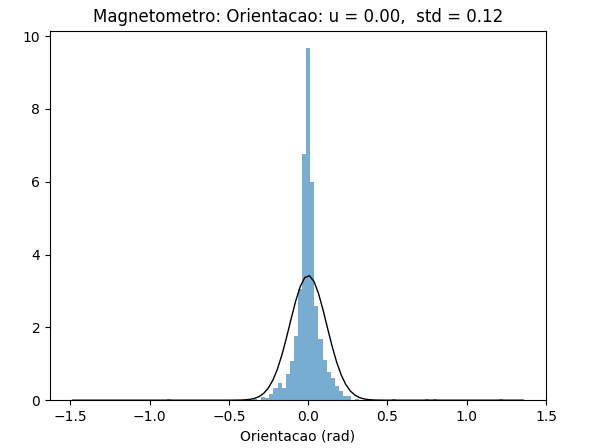
\includegraphics[width=0.7\textwidth]{mag_gaussiana}
\end{center}
\end{figure}
O magnetômetro também possui ruído aproximadamente gaussiano. A covariância encontrada foi 0.01356513.
\par
Utilizando os valores medidos dos encoders, giroscópio e magnetômetro, foi formada a matriz de covariância R:
\[
\begin{bmatrix}
	0.01356513 & 0 & 0 & 0\\
	0 & 4.53759819e-02 & 0 & 0\\
	0 & 0 & 3.05991867e-04 & 0\\
	0 & 0 & 0 & 3.92135776e-04\\
\end{bmatrix}
\]
\section{Covariância dos dados da visão computacional}
Aplicou-se 0.15m/s nas duas rodas para fazer o robô andar lentamente em linha reta em uma distância de aproximadamente 1 metro. Durante o movimento, foram armazenados os valores medidos pela visão computacional de posição (x, y) em metros e orientação ($\theta$) em radianos. Os valore medidos podem ser vistos no gráfico:
\begin{figure}[H]
	\caption{Posição e orientação medidos pela visão computacional, enquanto robô anda em linha reta}
\begin{center}
   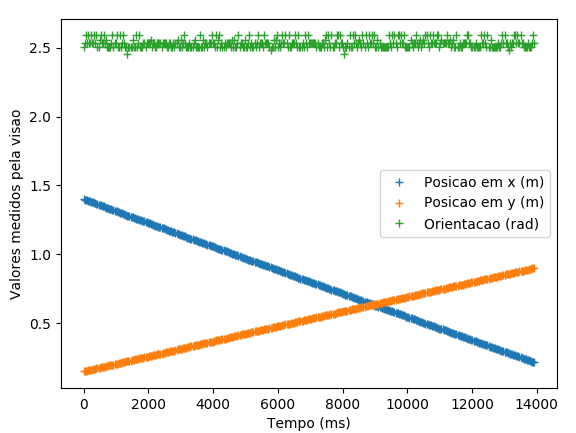
\includegraphics[width=0.7\textwidth]{visao}
\end{center}
\end{figure}
Para diferenciar a variação devido ao movimento do robô da variação devido ao ruído, foi calculado a regressão linear de x e y e, utilizando a equação de reta encontrada, foi subtraído o valor medido do valor ideal, mantendo apenas o ruido gaussiano branco. O histograma com fitting de gaussiana em x, y e $\theta$ são:
\begin{figure}[H]
	\caption{Ruido de posição no eixo x da visão computacional}
\begin{center}
   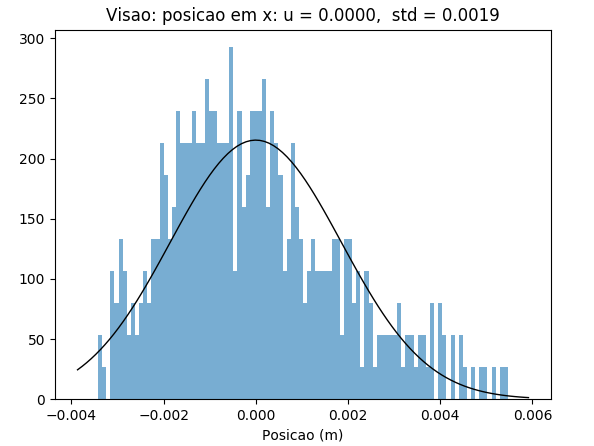
\includegraphics[width=0.7\textwidth]{visao_x_gaussiana}
\end{center}
\end{figure}
\begin{figure}[H]
	\caption{Ruido de posição no eixo y da visão computacional}
\begin{center}
   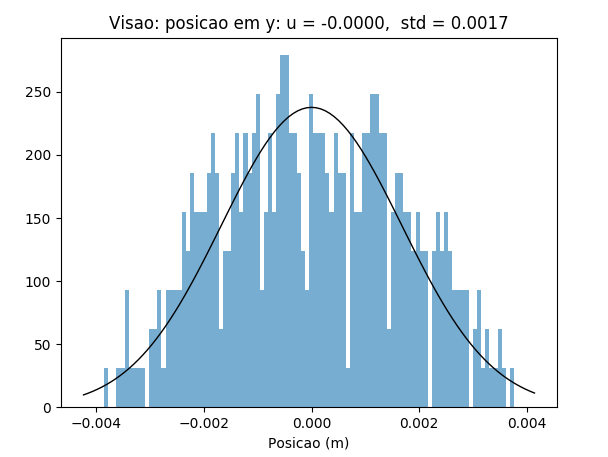
\includegraphics[width=0.7\textwidth]{visao_y_gaussiana}
\end{center}
\end{figure}
\begin{figure}[H]
	\caption{Ruido de orientação da visão computacional}
\begin{center}
   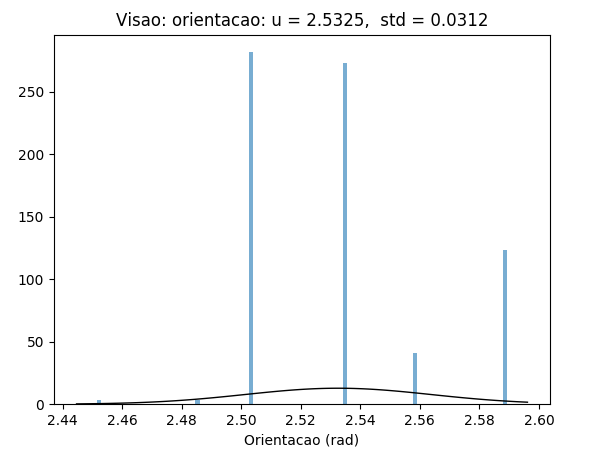
\includegraphics[width=0.7\textwidth]{visao_theta_gaussiana}
\end{center}
\end{figure}
Estes resultados indicam que não há grande resoluçao na medição de orientação, mas as de posição foram muito próximas de uma gaussiana. Já a coviariancia do offset do magnetômetro é a soma da covariancia da visão somada a covariancia do magnetômetro, resultando em 0.0145424.
Utilizando estes testes, foi obtida a matriz de covariança $R_v$:
\[
\begin{bmatrix}
	3.44048681e-06 & 0 & 0 & 0\\
	0 & 2.82211659e-06 & 0 & 0\\
	0 & 0 & 9.77316323e-04 & 0\\
	0 & 0 & 0 & 0.0145424\\
\end{bmatrix}
\]

\section{Matriz de ruído de processo $Q_t$}
A matriz de ruído de processo Q foi modelada como:
\[
\begin{bmatrix}
	Tk_x & 0 & 0 & 0 & 0 & 0 & 0\\
	0 & Tk_y & 0 & 0 & 0 & 0 & 0\\
	0 & 0 & Tk_\theta & 0 & 0 & 0 & 0\\
	0 & 0 & 0 & Tk_v & 0 & 0 & 0\\
	0 & 0 & 0 & 0 & Tk_\omega & 0 & 0\\
	0 & 0 & 0 & 0 & 0 & Tk_{\theta_{offset}} & 0\\
	0 & 0 & 0 & 0 & 0 & 0 & Tk_{\theta_y}\\
\end{bmatrix}
\]
Onde T é o período de amostragem e $k_i $ são constantes que devem ser ajustadas. Foi utilizado o período de amostragem porque quanto maior o tempo entre as iterações, maior é o erro no modelo.
\par
Quando a aceleração angular era modelada como constante, foi observado problemas com variações rápidas em $\omega$. Para observar os efeitos de $k_\omega$, os valores de velocidade angular foram medidas aplicado alternadamente 0.6m/s e -0.6m/s em cada roda. Com $k_\omega$ = 0.01, a estimativa do EKF é:
\begin{figure}[H]
	\caption{Velocidade angular estimada e medida, $k_\omega$ = 0.01}
\begin{center}
   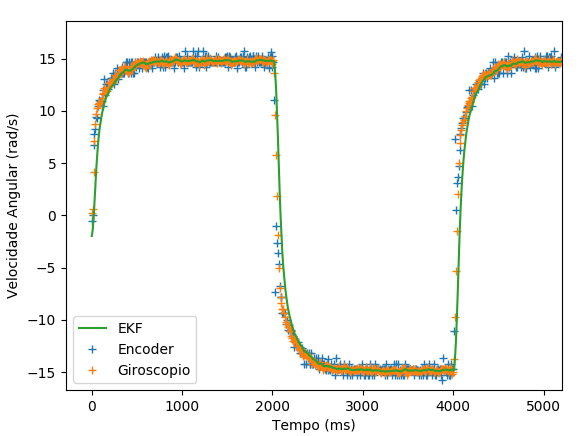
\includegraphics[width=0.7\textwidth]{process_noise_01_2}		
\end{center}
\end{figure}
Pode-se perceber que o filtro não conseguiu acompanhar bem as variações bruscas na velocidade angular. Este problema foi corrigido no modelo de aceleração constante utilizando um valor maior da constante, de $k_\omega$ = 0.1:
\begin{figure}[H]
	\caption{Velocidade angular estimada e medida, $k_\omega$ = 0.1}
\begin{center}
   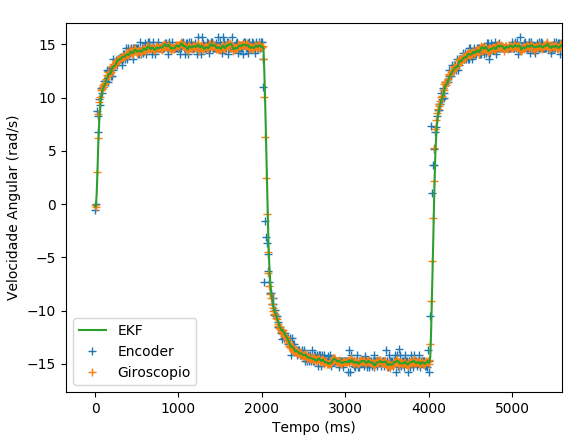
\includegraphics[width=0.7\textwidth]{process_noise_1_2}
\end{center}
\end{figure}
Neste novo teste, o ajuste no $k_\omega$ conseguiu melhorar muito a estimativa da velocidade angular mesmo durante as variações bruscas, por fazer o EKF confiar mais nas novas medidas e menos no valor predito a partir da estimativa anterior.
\par
Quando a aceleração foi levada em consideração no modelo utilizando a derivação numérica das velocidades das rodas, os problemas foram corrigidos. Mesmo para valores baixos de $k_\omega$, como 0.001, a estimativa conseguiu acompanhar corretamente os sensores:
\begin{figure}[H]
	\caption{Velocidade angular estimada e medida, $k_\omega = 0.001$}
\begin{center}
   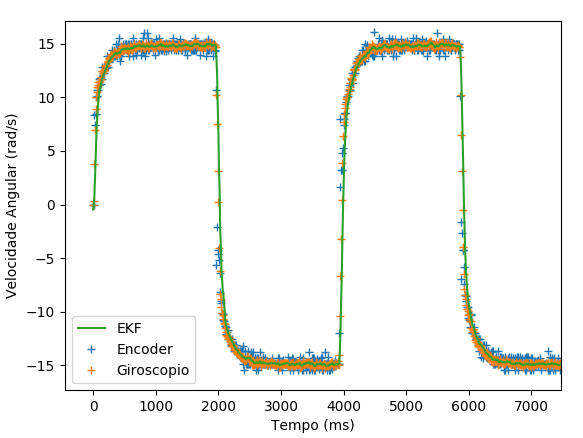
\includegraphics[width=0.7\textwidth]{process_noise_acc_2}
\end{center}
\end{figure}
\par
A orientação foi bem estimada com $k_\theta = 0.001$, como pode ser vista no gráfico:
\begin{figure}[H]
	\caption{Velocidade angular estimada e medida, $k_\theta = 0.001$}
\begin{center}
   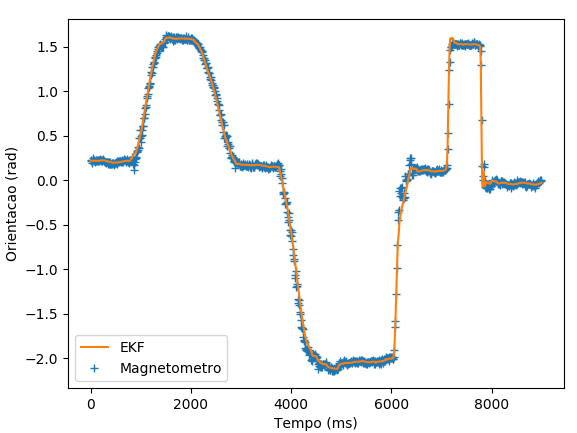
\includegraphics[width=0.7\textwidth]{mag_90_ekf}
\end{center}
\end{figure}
Neste teste, o robô foi girado manualmente por aproximadamente 90 graus, retornado para a orientação anterior, depois o movimento foi repetido na outra direção. Por fim, ele foi movimentado rápidamente, e o EKF continuou realizando boas estimativas.
\par
As constantes $Tk_{\theta_{offset}}$ e $Tk_{\theta_y}$ foram ajustadas para 0.005 e 0.0001 respectivamente por tentativa e erro, ajustando seus valores até que as estimatimativas ficassem adequadas.

\section{Unscented Kalman Filter}
Unscented Kalman Filter \cite{wan2000unscented}, ou UKF, é uma alternativa ao EKF que lineariza melhor o sistema. Em vez de linearizar o sistema utilizando aproximação de Taylor de primeira ordem como o EKF faz, o UKF gera vários pontos (chamados de pontos sigma) próximos ao valor real, os passa pelo modelo do sistema e gera uma estimativa final, aplicando pesos a cada um desses pontos. Dessa forma, o UKF propaga a covariancia pelo modelo não linear alcançando precisão de terceira ordem para qualquer não linearidade.
\par
Assim como o EKF, o UKF tem uma etapa de prediçao. Primeio, os pontos sigma são gerados:
\begin{equation}
	X_{0} = x
\end{equation}
\begin{equation}
	X_{i} = x + (\sqrt{(L + \lambda) \Sigma})_i, i = 0,..,L
\end{equation}
\begin{equation}
	X_{i} = x - (\sqrt{(L + \lambda) \Sigma})_{i - L}, i = L + 1,.., 2L
\end{equation}
Em que X é uma matriz de tamanho 2L + 1 x L, x é o vetor de variáveis de estado e $X_i$ é a i-ésima coluna de X.
Depois a predição é calculada para cada ponto sigma:
\begin{equation}
	X_t = F(X_{t-1})
\end{equation}
E então os pontos sigmas preditos são utilizados para calcular a nova covariancia e as novas variáveis de estado:
\begin{equation}
	x_t = \sum\limits_{i=0}^{2L} W_i* X_{i, t}
\end{equation}
\begin{equation}
	\Sigma = \sum\limits_{i=0}^{2L} W_i * [X_{i, t} - x_t] [X_{i, t} - x_t]^T
\end{equation}
A etapa de atualização é semelhante. Os pontos sigmas são gerados e calcula-se as leituras preditas através do modelo de medidas:
\begin{equation}
	Y_t = H(X_t)
\end{equation}
\begin{equation}
	y_t = \sum\limits_{i=0}^{2L} W_i* Y_{i, t}
\end{equation}
E depois é calculado as variáveis de estado e suas covariancias:
\begin{equation}
	\Sigma_{y,y} = \sum\limits_{i=0}^{2L} W_i * [Y_{i, t} - y_t] [Y_{i, t} - y_t]^T
\end{equation}
\begin{equation}
	\Sigma_{x,y} = \sum\limits_{i=0}^{2L} W_i * [X_{i, t} - x_t] [Y_{i, t} - y_t]^T
\end{equation}
\begin{equation}
	K = \Sigma_{x,y} \Sigma_{y,y}^{-1}
\end{equation}
\begin{equation}
	x_t = x_t + K (y_{medido, t} - y_t)
\end{equation}
\begin{equation}
	\Sigma_t = \Sigma_t - K  \Sigma_{y,y} K^{T}
\end{equation}
As constante $\lambda$ define a distancia entre os pontos sigma e o centro, e as constantes $W_i$ são pesos aplicados a cada ponto sigma.

\section{Comparação como o UKF}
O UKF requer mais memoria do microcontrolador, já que precisa armazenar uma matriz com todos os pontos sigmas durante sua execução, enquanto o EKF só armazena as variáves de estado, que é um vetor menor ((2L+1) x L para o UKF vs Lx1 para o EKF, em que L é o numero de variáveis de estado. 
\par
Também houveram mais dificuldades de implementá-lo no microcontrolador, devido ao calculo de raíz quadrada da matriz de covariancia, que causou erros de execução se as constantes não estivessem bem ajustadas. Esses erros eram devido a matriz de covariancia deixar de ser positiva semi-definida, o que tornava impossível calcular sua raíz quadrada. Esses problemas foram resolvidos por tentativa e erro, ajustando as constantes até não houvessem mais erros.
\par
O UKF também é computacionalmente mais pesado. O tempo total gasto calculando uma etapa inteira de predição e atualização foi maior que o EKF:
\begin{center}
\begin{tabular}{ | l | l | l | p{5cm} |}
    \hline
    Algoritmo & Tempo (ms) \\ \hline
    EKF & 1.3 \\ \hline
    UKF & 6.3 \\
    \hline
\end{tabular}
\end{center}
Esse peso computacional é uma desvantagem comparado ao EKF caso seja utilizado em um sistema que exija um controlador com períodos menores. O controlador do robô utilizado tem um período de 10 ms, então isso não foi um problema. Esse peso computacional também resulta em valores menores lidos de cada sensor. Isso resulta na perda de muitas leituras do giroscópio, que é capaz de obter uma nova medida a cada 0.6 ms, e do acelerômetro.
\par
Suas estimativas foram comparadas enquanto o robô realizava um movimento circular, aplicando uma velocidade na roda direita de 0.6 m/s e na roda direita de 0.5 m/s. Os erros em x, y e $\theta$ foram medidos a cada atualização do EKF e do UKF. A variação do erro em $\theta$ foi:
\begin{figure}[H]
  \centering
  \begin{minipage}[b]{0.45\textwidth}
    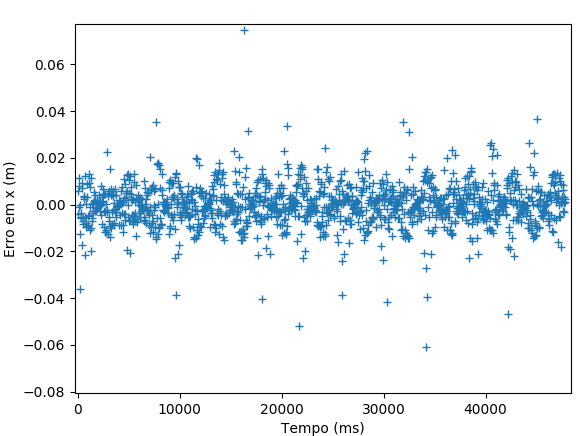
\includegraphics[width=\textwidth]{ukf_x}
    \caption{Erro em x do UKF}
  \end{minipage}
  \begin{minipage}[b]{0.45\textwidth}
    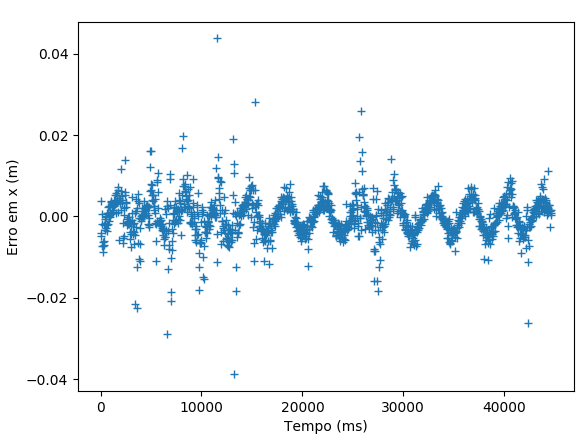
\includegraphics[width=\textwidth]{ekf_x}
    \caption{Erro em x do EKF}
  \end{minipage}
\end{figure}
\begin{figure}[H]
  \centering
  \begin{minipage}[b]{0.45\textwidth}
    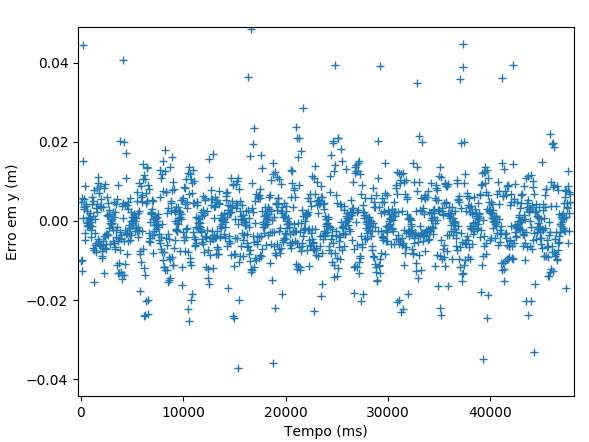
\includegraphics[width=\textwidth]{ukf_y}
    \caption{Erro em y do UKF}
  \end{minipage}
  \begin{minipage}[b]{0.45\textwidth}
    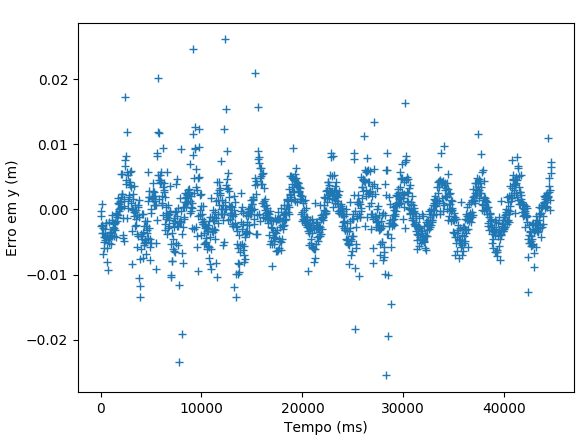
\includegraphics[width=\textwidth]{ekf_y}
    \caption{Erro em y do EKF}
  \end{minipage}
\end{figure}
\begin{figure}[H]
  \centering
  \begin{minipage}[b]{0.45\textwidth}
    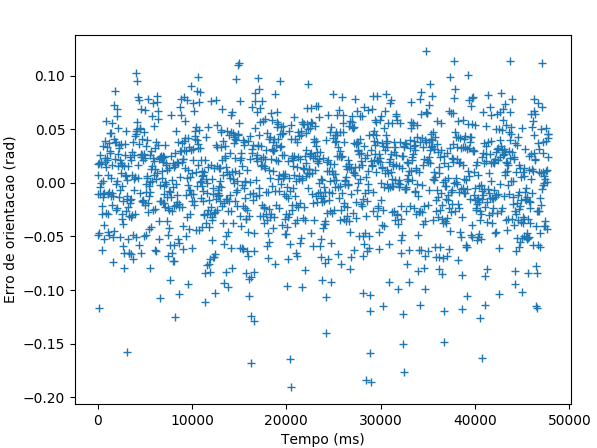
\includegraphics[width=\textwidth]{ukf_theta_comp}
    \caption{Erro de orientação do UKF}
  \end{minipage}
  \begin{minipage}[b]{0.45\textwidth}
    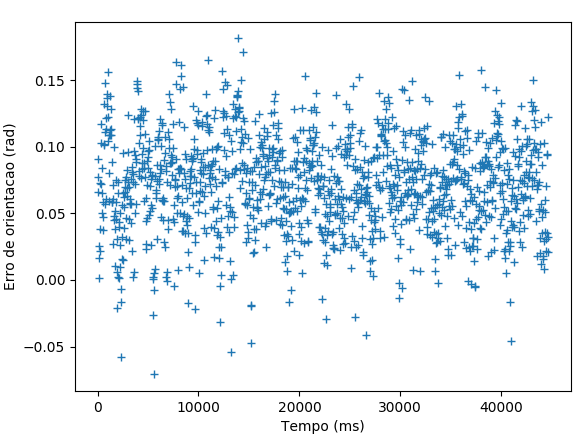
\includegraphics[width=\textwidth]{ekf_theta_comp}
    \caption{Erro de orientação do EKF}
  \end{minipage}
\end{figure}
A média dos erros observados foram:
\begin{center}
\begin{tabular}{ | l | l | l | p{5cm} |}
    \hline
    Variável & EKF & UKF \\ \hline
    x (m) & 0.0041313 & 0.0067911 \\ \hline
    y (m) & 0.0033865 & 0.0064115 \\ \hline
    $\theta$ (rad) & 0.0723554	& 0.0360838 \\
    \hline
\end{tabular}
\end{center}
O UKF estimou melhor a orientação, mas obteve resultados inferiores ao estimar a posição em x e y. A causa provável do UKF não ter obtido o desempenho superior em todas as estimativas é a menor taxa de atualização, que o faz corrigir suas estimativas 5 vezes menos frequentemente.

% ---
% primeiro capitulo de Resultados
% ---
\chapter{Resultados}
% ---
Movimentando o robô manualmente mostra que o EKF consegue estimar bem o ângulo do robô:
\begin{figure}[H]
	\caption{Estimativa de orientação e velocidade angular}
\begin{center}
   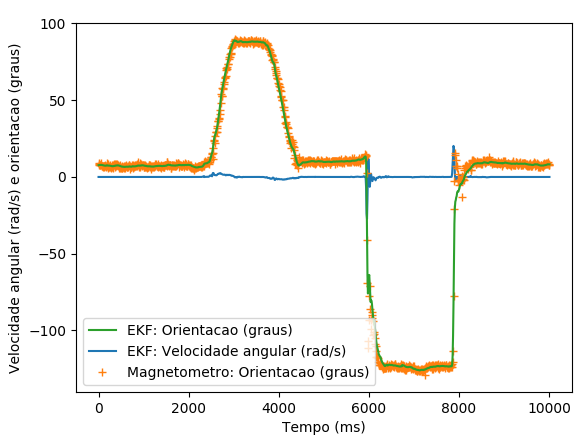
\includegraphics[width=0.7\textwidth]{ekf_theta}
\end{center}
\end{figure}
Na segunda vez que o robô foi girado, a velocidade angular aplicada foi maior que o giroscópio consegue medir. Apesar disso, o magnetômetro foi capaz de ajustar a estimativa de orientação corretamente. Visualizando a estimativa no segundo giro:
\begin{figure}[H]
	\caption{Comparação dos valores medidos e estimados da orientação}
\begin{center}
   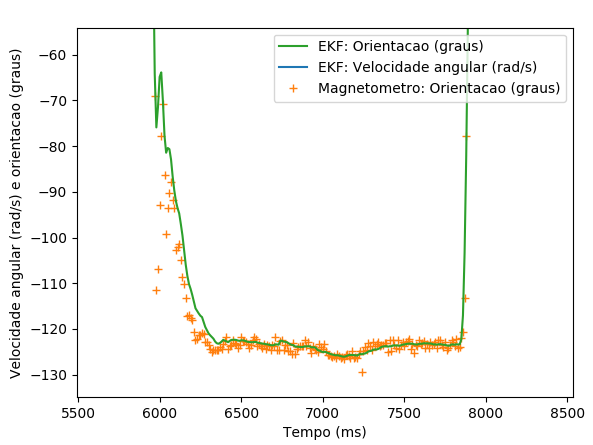
\includegraphics[width=0.7\textwidth]{ekf_theta_proximo}
\end{center}
\end{figure}
É possível perceber o atrazo na estimativa devido a saturação do giroscópio, e apesar disso o valor estimado ainda converge para o valor real devido as correções do magnetômetro. Também é visível que a rejeição de ruídos resulta numa estimativa muito estável.
\par
Ao utilizar os dados da visão computacional, o EKF converge rapidamente para a posição e orientação correta devido a alta covariancia inicial, mesmo com posição inicial em (0, 0, 0):
\begin{figure}[H]
	\caption{Convergencia aos valores medidos pela visão computacional}
\begin{center}
   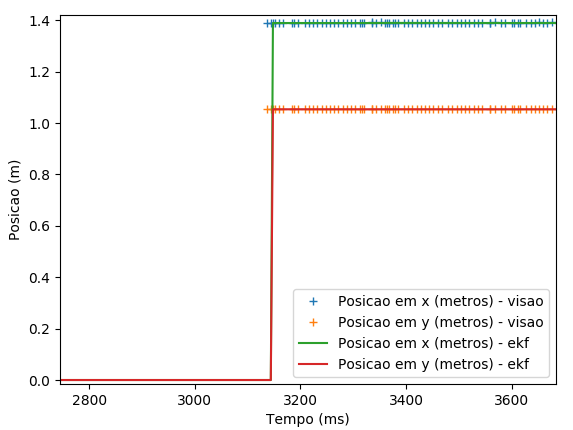
\includegraphics[width=0.7\textwidth]{ekf_vision_conv}
\end{center}
\end{figure}
No mesmo gráfico podem ser vistas algumas medidas incorretas de orientação provenientes da visão computacional, que não influenciaram muito na estimativa.
\par
O robô foi movimentado manualmente sem que as rodas girem, de forma que o encoder não consiga detectar o movimento do robô. Após algumas medidas, a estimativa convergiu para o valor correto através das correções fornecidas pelos dados de visão:
\begin{figure}[H]
	\caption{Estimativa de posicão enquanto as rodas derrapam (tempo em dezenas de ms)}
\begin{center}
   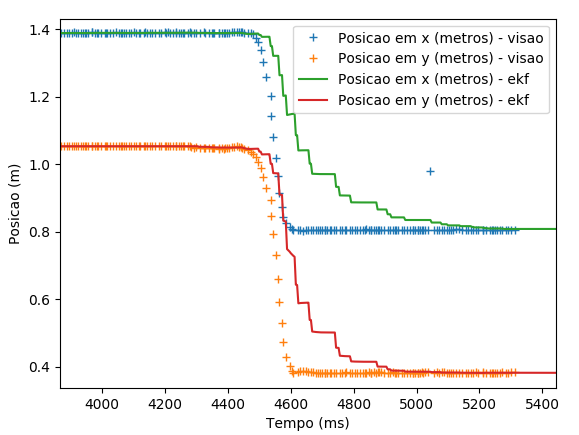
\includegraphics[width=0.7\textwidth]{ekf_pos_manual}
\end{center}
\end{figure}
\par
O que indica que derrapamentos não causarão erros permanentes nas estimativas.
\par
Ao fazer um movimento circular, as posições estimadas e da visão são:
\begin{figure}[H]
	\caption{Medidas e estimativa de posição, movimento circular}
\begin{center}
   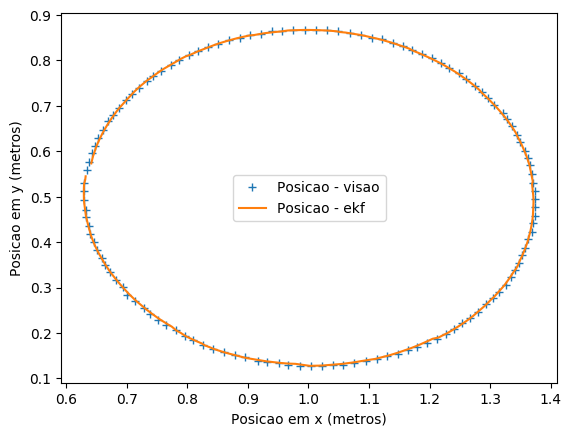
\includegraphics[width=0.7\textwidth]{ekf_circular}
\end{center}
\end{figure}
O erro é pequeno. A distancia entre a posição estimada e a obtida pela visão é:
\begin{figure}[H]
	\caption{Distancia entre estimativas e visão computacional}
\begin{center}
	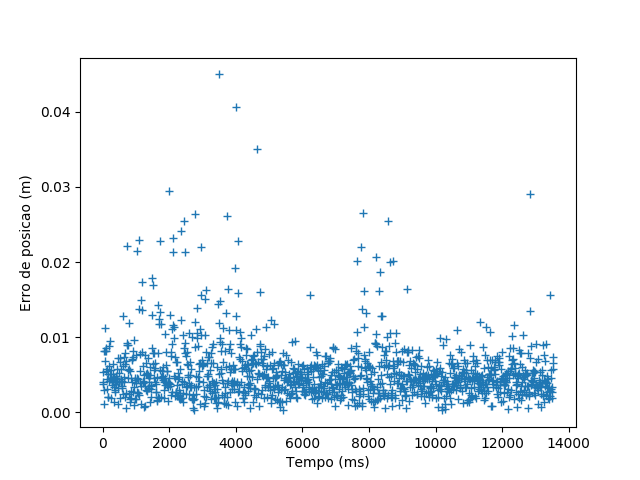
\includegraphics[width=0.7\textwidth]{ekf_circular_erro2}
\end{center}
\end{figure}
\par
Com média de 0.532 cm.
\par
Ao testar o sistema de controle já presente no robô, utilizando as estimativas do EKF em vez da odometria utilizada anteriormente, foi notado um aumento significativo da estabilidade do sistema. Sem o EKF, não era possível controlar o robô mandando novos comandos a velocidade máxima (33 ms), exigindo delays de 200 ms a cada comando. Isto indica que a obtenção de estimativas mais precisas e com menos erros causados por derrapamentos é uma boa solução para os problemas de controle descritos anteriormente.

\section{Atendimento do cronograma}
No planejamento inicial do primeiro semestre, foram definidas as seguintes atividades:
\begin{itemize}
	\item Pesquisa bibliográfica e desenvolver modelo do robô
	\item Escrever algoritmo do Filtro de Kalman e testar no robô
	\item Estudar propriedades de cada sensor e configurá-los
	\item Medir ruído dos sensores e adicionar dados ao filtro
	\item Testar estimativas do algoritmo
	\item Fazer melhorias, corrigir problemas e testar outros modelos
\end{itemize}

Foi possível fazer todos a tempo, mas algumas foram mais difíceis e demoradas do que o esperado, enquanto outras foram mais fáceis. 
O desenvolvimento do modelo inicial do robô foi relativamente rápido, porque o robô já foi estudado pela literatura suficientemente bem. O modelo utilizado neste projeto é muito comun na literatura.
\par
A primeira implementação do EKF e sua execução no robô, feita inicialmente com representação de ponto fixo, foi terminada mais rápido do que esperado, mas foi refeita posteriormente para alcançar precisão melhor, o que exigiu mais tempo.
\par
Já a configuração dos sensores foi a parte que mais levou tempo. Não houve dificuldades para implementar a leitura dos sensores, mas a presença de diversas distorções nos sensores exigiu tempo adicional para corrigi-las. Cada sensor teve que ser testado e configurado multiplas vezes, encontrando problemas e os corrigindo.
\par
As ultimas atividades de medir ruídos, testar as estimativas e fazer melhorias foram realizadas de forma iterativa. Algumas medidas de estimativas demonstraram bugs na implementação EKF, outras mostraram que algumas correções no modelo eram necessárias, e outras que era as calibrações de alguns sensores que foram melhoradas.

Já no segundo semestre, foi definida as atividades:
\begin{itemize}
	\item Estudar acelerômetro e implementar leitura dos dados
	\item Modificar modelo do robô para adicionar dados de aceleração
	\item Corrigir distorções do acelerômetro e ajustar covariâncias
	\item Corrigir distorções do magnetômetro e testes
	\item Comparação com o UKF
\end{itemize}
Todas as atividades foram concluídas. A implementação da leitura dos dados do acelerômetro foi feita rapidamente, devido a sua similaridade com os outros sensores. Adicionar o acelerômetro não exigiu muitas mudanças iniciais ao modelo do robô, já que já eram utilizados dados de aceleração através da velocidade das rodas.
\par
Já a correção de distorçoes do acelerômetro foi a parte mais problemática. A variação de inclinação do robô no eixo y dificultou a remoção dos efeitos da gravidade no acelerômetro, exigindo que a inclinação do robô também fosse estimada pelo EKF. Já os efeitos da aceleração centrípeta foram mais simples de remover devido a presença do giroscópio. No final, as distorções encontradas foram removidas e o acelerômetro ficou adequado ao uso no sistema.
\par
A correção das distorções do magnetômetro exigiu apenas pequenas mudanças no modelo de medidas dos sensores e ajustes em constantes das matrizes de covariancia e de ruído de processo. As correções implementadas resolveram os problemas encontrados no primeiro semestre.
\par
Já a implementação do UKF resultou em muitos problemas. O UKF exige mais memória e processamento do microcontrolador, o que precisou de mais cuidado em sua implementação. Além disso, o calculo de raíz quadrada da matriz de covariancia causava erros de execução se as constantes não fossem bem ajustadas, porque constantes mal ajustadas faziam a matriz de coviariancia deixar de ser positiva semi-definida. Apesar dos problemas, o UKF foi implementado e a comparação foi realizada.

% ----------------------------------------------------------
% Finaliza a parte no bookmark do PDF
% para que se inicie o bookmark na raiz
% e adiciona espaço de parte no Sumário
% ----------------------------------------------------------
\phantompart

% ---
% Conclusão
% ---
\section{Conclusão}
\par

O projeto realizado alcançou seus objetivos e conseguiu uma boa estimativa das variáveis de estado. Os valores estimados apresentam boa rejeição de ruído e rápida recuperação de leituras incorretas, resultando em estimativas mais robustas do que soluções com sensores trabalhando de forma individual.
\par
Os sensores necessitaram de diversos ajustes, como a de remoção de interferências no magnetômetro, remoçao de componentes indesejadas nas medidas do acelerômetro como a aceleração da gravidade e centrípeta, ajustes em distorções no giroscópio. Esses ajustes foram corrigidos, permitindo um bom uso dos sensores.
\par
A comparação com o UKF obteve resultados mistos: a estimativa de algumas variáveis melhoraram, enquanto outras pioraram. Este resultado podem ser causado pelo desempenho inferior do microcontrolador ao calcular o UKF, e devem ser melhorados caso um microcontrolador de maior capacidade de processamento seja utilizado.
\par

% ---

% ----------------------------------------------------------
% ELEMENTOS PÓS-TEXTUAIS
% ----------------------------------------------------------
\postextual
% ----------------------------------------------------------

% ----------------------------------------------------------
% Referências bibliográficas
% ----------------------------------------------------------
\bibliography{referencias.bib}

% ----------------------------------------------------------
% Glossário
% ----------------------------------------------------------
%
% Consulte o manual da classe abntex2 para orientações sobre o glossário.
%
%\glossary

%---------------------------------------------------------------------
% INDICE REMISSIVO
%---------------------------------------------------------------------
\phantompart
\printindex
%---------------------------------------------------------------------

\end{document}
